\documentclass[12pt,a4paper,titlepage]{scrartcl}
\usepackage[left=3cm,right=4cm,top=3cm,bottom=3cm,includeheadfoot]{geometry}
\usepackage{german}
\usepackage{graphicx}

\usepackage{color}
\usepackage{amsmath}
\usepackage{amssymb}
\usepackage{polynom}
\usepackage{array}
\usepackage[table]{xcolor}
\usepackage[colorlinks,pdfpagelabels,pdfstartview = FitH,bookmarksopen = true,bookmarksnumbered = true,linkcolor = black,plainpages = false,hypertexnames = false,citecolor = black]{hyperref}
\usepackage{fancyhdr}

%Serifenschrift in Überschrift
%\usepackage{sectsty}
%\allsectionsfont{\rmfamily}
%\usepackage{tocloft}
%\renewcommand{\cftsecfont}{\rmfamily}
%\renewcommand{\cftsecfont}{\bfseries}

%Plots
\usepackage{tkz-euclide}
\usetikzlibrary{calc}
\usepackage{pgfplots}
\usepackage{tikz}
\usetikzlibrary{calc,trees,positioning,arrows,fit,shapes,calc}
\newcounter{angle}
\setcounter{angle}{220}

%Polynomdivision
 \usepackage{polynom}
 \polyset{style=C, div=:,vars=x}

\pagestyle{fancy}
\fancyhf{}
\fancyhead[C]{Vorkurs (Mathematik)}
\renewcommand{\headrulewidth}{0.5 pt}
\fancyfoot[L]{\today}
\fancyfoot[C]{\thepage}
\fancyfoot[R]{FS07}
\renewcommand{\footrulewidth}{0.5 pt}
\newcommand{\psection}[1]{\pagebreak\section{#1}}
\definecolor{DarkGrey}{RGB}{128,128,128}

\newtheorem{remark}{Bemerkung}[section]
\newtheorem{axiom}{Satz}[section]
\newtheorem{definition}{Definition}[section]
\newtheorem{example}{Beispiel}[section]
\newtheorem{important}{Merke}[section]
\newtheorem{theorem}{Theorem}[section]

\definecolor{agreen}{rgb}{0.5,1.0,0.5}
\definecolor{ared}{rgb}{1.0,0.5,0.5}
\definecolor{blue}{rgb}{0.5,0.5,1.0}

\begin{document}
\pagenumbering{roman}
%\setkomafont{disposition}{\normalfont\rmfamily}
\addtokomafont{disposition}{\rmfamily}
\titlehead
{
 	\begin{flushright}
 		
\includegraphics[width = 7cm]{pictures/hm-logo.pdf}
 	\end{flushright}
 	 	\line(1,0){400}
}

\subject{\includegraphics*[width=9 cm]{pictures/fs-logo.pdf}}
\title{Vorkurs/Mathematik\linebreak}
\subtitle{Eine kompakte Vorbereitung der Mathematik des Informatikstudiums}
\author{von Stephan Plöderl}
\publishers{Fachschaft 07}
\date{\today}
\thispagestyle{empty}
\maketitle
\newpage
\setcounter{page}{1}
\tableofcontents
\newpage
\clearpage

\pagenumbering{arabic}
\psection{Einf"uhrung}
\subsection{Worum geht's im Vorkurs Mathematik?}
Jeder Studierende tut sich in unterschiedlichen F"achern unterschiedlich schwer.
Es gibt jedoch F"acher, in denen die Durchfallquote bereits "uber Jahre "uberdurchschnittlich hoch ist.
Bei einem dieser F"acher mit besonders hoher Durchfallquote handelt es sich um das mathematische Fach Analysis.
Aus diesem Grund haben wir als Fachschaft es uns so wie bereits einige vor uns zur Aufgabe gemacht, dem ganzen ein wenig entgegenzusteuern und zu versuchen, euch die Grundlagen die f"ur dieses Fach von N"oten sind zu vermitteln.

\subsection{An wen richtet sich dieser Kurs?}
Dieser Kurs richtet sich an all jene,
\begin{itemize}
\item welche Schwächen in mathematischen F"achern haben.
\item deren Schulzeit schon etwas länger her ist.
\item welche nicht von mathematisch/technischen Schulen bzw. Gymnasien kommen.
\item und an all jene welche der Meinung sind, eine Wiederholung schadet nie.
\end{itemize}

\subsection{Warum Mathematik im Informatikstudium?}
Vielen Studierenden ist nicht klar, warum Mathematik so grundlegend wichtig f"ur ihr Studium ist - schlie"slich studieren sie ja keine (reine) Mathematik! Dieses Kapitel soll jenes Verst"andnisproblem l"osen und aufzeigen, welche Schnittpunkte zwischen Mathematik und Informatik bestehen.\\
Mit Mathematik haben Informatiker ein zus"atzliches, sehr m"achtiges Werkzeug zur Hand, mit dem viele scheinbar unl"osbare Probleme pl"otzlich l"osbar werden.
Deshalb gibt es in der Informatik einige Bereiche in denen ein gewisses mathematisches Grundverst"andnis notwendig ist.\\
Im Folgenden möchten wir nun anhand einiger Beispiele den Nutzen von Mathematik-Kenntnissen im Bereich Informatik verdeutlicht:

\subsubsection{Spieleentwicklung}
Die Entwicklung eines Spiels umfasst neben der Programmierung noch sehr viele andere Bereiche, wie Psychologie, Design und Soziologie (um nur ein paar zu nennen). Auch die Mathematik spielt hierbei eine gro\ss e Rolle:\\
So ermöglicht es einem die (nummerische) Integration, dass sich Figuren realistischer Bewegen können.\\
Auch Lichteffekte wie Spiegelungen oder der Soundeffekte wie Widerhall m"ussen zuerst korrekt mathematisch beschrieben und dann implementiert werden, wenn sie \glqq realistisch\grqq wirken sollen.\\
Alle beschriebenen Probleme k"onnen mit relativ einfachen, mathematischen Methoden gel"ost werden.

\subsubsection{Business Analytics}
Business Analytics wird eingesetzt, um die Probleme in der Unternehmenswelt mittels Analyse gro\ss er Datenmengen (Big Data) zu l"osen.\\
Solche Probleme sind zum Beispiel die Ermittlung von \glqq Risikokunden\grqq, die unzufrieden sind und deshalb ihren Handyvertrag k"undigen wollen. 
K"onnen diese Kunden per Business Analytics gezielt ermittelt werden, so ist es möglich sie mit speziellen Angeboten, wie Freiminuten, von der K"undigung abzuhalten.\\
Die Ermittlung der Kunden erfolgt hierbei durch statistische Analysen wie Regression oder Decision Trees.

\subsubsection{Machine Learning}
Durch die immer schneller rechnenden Computer k"onnen heute Probleme gel"ost werden, die fr"uher nur Menschen erledigen konnten. Dazu geh"oren automatische Gesichtserkennung, das Auffinden von Tumoren in medizinischen Bildern oder die Erkennung von Kreditkartenbetrug. Meist steht hinter diesen Anwendungen das sogenannte \glqq Machine Learning \grqq, was bedeutet, dass die Maschine (der Computer) selbst lernt, welche Eigenschaften in den auftretenden Daten (Bilder von Gesichtern, Kreditkarten"uberweisungen, Bilder von Tumoren oder gesundem Gewebe) zu welchem Ergebnis passt (Gesichter werden bestimmten Menschen zugeordnet, eine "uberweisung wird als Betrug markiert, ein Gewebebild wird als gesund gekennzeichnet). Das praktische am selbstlernenden Computer: der Mensch muss nur noch eine sogenannte Trainingsmenge an Datenmaterial bereitstellen, an der der Computer lernen kann - nach dem Training ist die Maschine selbst"andig in der Lage, eine Zuordnung zu machen.
Diese selbstlernenden Programme basieren auf mathematische Grundlagen.\\
Einen hierfür oft verwendeten Ansatz bieten die sogenannten \glqq neuronalen Netze\grqq.
Welche wiederum auf  Ma\-trix/\-Vektor-\-Multiplikationen beruhen.\vspace{0.5cm}\\
Alle mathematischen Grundkenntnisse, welche in diesen und weiteren Bereichen ben"otigt werden, k"onnen im Studium erlernt werden.


\psection{Aussagenlogik}
Die Logik "offnete den Weg f"ur die Informatik. Sie war immer eine Disziplin der Philosophie und hat eine sehr interessante Geschichte (von Aristoteles, Kant, Hegel, Boole, Russell, Gentzen, Skolem, G"odel, bis zu Turing und weiter) hinter sich gelassen. Die Aussagenlogik als kleiner aber grundlegender Teil ist intuitiv und auf sehr nat"urliche Weise begreifbar. Sie ist fundamental um mathematische Ausdr"ucke zu verstehen und wird in allen Bereichen der Mathematik verwendet. In der Informatik hat die Logik und damit auch die Aussagenlogik eine wichtige Bedeutung. In der technischen Informatik werden Kodierer und Dekodierer, Addierer und Multiplizierer mit sogenannten logischen Gattern realisiert. Ein Gatter ist nichts anders als eine logische Verkn"upfung. Zum Beispiel ist das Und-Gatter ein Gatter mit zwei Eing"angen $x_{in}^1, x_{in}^2$ und einem Ausgang $x_{out}$ mit 
\begin{equation*}
	x_{out} = x_{in}^1 \land x_{in}^2.
\end{equation*}
Legt man nun eine gewisse Spannung an $x_{in}^1$ und \textit{gleichzeitig} $x_{in}^2$ an, so gibt das Gatter diese Spannung weiter, ansonsten nicht. Die Gatter bilden den Kern der Computerhardware wie z.B. Mikroprozessoren. Zudem ist die Aussagenlogik in jeder Programmiersprache eingebettet. Sie werden viele logische Ausdr"ucke in Java schreiben.

Sp"ater im Studium werden die meisten von Ihnen das Konzept einer formalen Sprache kennenlernen. Formale Sprachen und bestimmte Teile der Logik sind sehr eng miteinander verbunden. Die aktuelle Forschung besch"aftigt sich mit der automatisierten Beweis"uberpr"ufung und sogar mit dem automatisierten Beweisen bisher unbewiesener Aussagen. Die Logik ist zudem im Bereich k"unstliche Intelligenz und Robotik essentiell. Und: ein bisschen Logik kann auch f"ur den Alltag nicht schaden.

Wir werden die Aussagenlogik besprechen und einen ganz kurzen ersten Blick auf die Pr"adikatenlogik werfen. Beherrschen sie diese beiden Bereiche der Logik, so sind sie f"ur das gesamte Bachelorstudium gewappnet.

%\subsection{Alles auf Anfang}
%Ein mathematisches System baut auf gewissen Grundregeln auf, die nicht bewiesen werden k"onnen und intuitiv gew"ahlt werden (meist durch Beobachtungen aus der Natur). Ohne Grundregeln k"onnte man keine Folgerungen aufstellen. Das hei{\ss}t aber auch, dass wir uns immer im Hinterkopf halten m"ussen, dass wenn diese Regeln in sich zusammenbrechen, auch das gesamte System zusammenbricht. Eine absolute Wahrheit ist also nicht bekannt. Dies mag zun"achst sehr unbefriedigend klingen aber die Resultate aus der Mathematik haben sich bisher als wahr herausgestellt, eine absolute Gewissheit existiert allerdings nicht!

\subsection{Aussagenlogik}
\begin{definition}[Aussage]
Eine Aussage ist ein als Satz formulierter Gedanke, dem man auf sinnvolle Weise einen Wahrheitswert zuordnen kann.
\end{definition}
%\begin{axiom}[Gesetz vom ausgeschlossenen Dritten]
Eine Aussage ist entweder \textbf{wahr (w)} oder \textbf{falsch (f)} (Gesetz vom ausgeschlossenen Dritten).
%\end{axiom}

\subsubsection*{Beispiele}
\begin{itemize}
\item $A_1 := $ Die Sonne strahlt w"arme ab.
\item $A_2 := $ Bayern M"unchen wird diese Saison wieder deutscher Meister.
\item $A_3 := 1+1 = 2$
\item $A_4 := $ Wird in diesem Jahr Ostern gefeiert?
\end{itemize}
$A_1$ und $A_3$ sind offensichtlich wahre Aussagen. $A_2$ k"onnen wir derzeit nicht "uberpr"ufen, sie ist aber trotzdem wahr oder falsch und darum zul"assig. $A_4$ ist keine Aussage, sondern eine Frage - die Antwort darauf kann wieder eine Aussage sein (z.B. \textit{In diesem Jahr wird Ostern gefeiert.}).

\subsubsection*{Schreibweisen}
Wir schreiben gew"ohnlich $A$ ist \textbf{wahr} oder \textbf{falsch}, \textbf{w} oder \textbf{f} bzw. (f"ur uns Informatiker) \textbf{1} oder \textbf{0}.

\subsubsection{Logische Verkn"upfungen}
\begin{definition}[Negation]
Unter der Negation einer Aussage $A$ versteht man die Aussage $\neg A$ (Mathe) bzw. $\overline{A}$ (Informatik) (in Worten:\glqq nicht $A$\grqq ), die genau dann wahr ist, wenn $A$ selbst falsch ist.
\end{definition}
Es folgt eine sogenannte \textbf{Wahrheitstabelle} der Verkn"upfung. In der ersten Spalte stehen die Werte, die $A$ annimmt, und in der rechten Spalte, Werte, die $\neg A$ dann besitzt. Solche Wahrheitstabellen werden Sie in der technischen Informatik viele erstellen. Besitzt eine logische Verkn"upfung bzw. eine aussagenlogische Formel $k$ verschiedene Variablen, so gibt es $2^k$ verschiedene Belegungen. Dabei bedeutet, Belegung, dass jede Variable bzw. Aussage entweder wahr oder falsch ist. Jede Aussage kann 2 Werte annehmen bei $k$ Aussagen sind das $\underbrace{2 \cdot 2 \cdot \cdots \cdots 2}_{k-\text{mal}} = 2^k$ M"oglichkeiten.
\begin{center}
\begin{tabular}{c||c}
 $A$ & $\neg A$  \\ 
\hline
\cellcolor{ared}falsch  & \cellcolor{agreen}wahr   \\ 
\cellcolor{agreen}wahr  & \cellcolor{ared} falsch  \\ 
\hline
\end{tabular}
\end{center}

\paragraph*{Beispiel:}
\begin{itemize}
	\item Die Negation der Aussage \glqq 4 ist ungerade\grqq \ ist die Aussage \glqq 4 ist gerade\grqq , denn es gibt nur diese beiden M"oglichkeiten.
	\item Aber die Negation der Aussage \glqq 4.5 ist ungerade\grqq \ ist nicht die Aussage \glqq 4.5 ist gerade\grqq, denn beide Aussagen sind falsch, ja sogar unsinnig. Die Negation der Aussage \glqq Diese Kuh ist schwarz\grqq \ ist nicht etwa die Aussage \glqq Diese Kuh ist wei{\ss}\grqq , denn es gibt ja noch andere Farben. Vielmehr m"usste man sagen:\glqq Diese Kuh ist nicht schwarz\grqq. Das umgangssprachliche Gegengenteil ist meist etwas anderes als die logische Verneinung.
\end{itemize}

\begin{definition}[Konjunktion]
Unter der Konjunktion zweier Aussagen $A$ und $B$ versteht man die Aussage $A \land B$ (Mathe) bzw. $A \cdot B$ (Informatik) (in Worten:\glqq $A$ und $B$\grqq ), die genau dann wahr ist, wenn $A$ und $B$ gleichzeitig wahr sind.
\end{definition}
In den ersten Spalten dieser \textbf{Wahrheitstabelle} stehen die Werte der Variablen der Konjunktion, in der letzten Spalte der resultierende Wert.
\begin{center}
\begin{tabular}{c|c||c}
 $A$& $B$  &  $A \land B$  \\ 
\hline
\cellcolor{ared} falsch & \cellcolor{ared} falsch & \cellcolor{ared} falsch   \\ 
\cellcolor{ared} falsch & \cellcolor{agreen} wahr & \cellcolor{ared} falsch  \\ 
\cellcolor{agreen} wahr & \cellcolor{ared} falsch & \cellcolor{ared} falsch   \\ 
\cellcolor{agreen} wahr & \cellcolor{agreen} wahr & \cellcolor{agreen} wahr  \\ 
\hline
\end{tabular}
\end{center}

\paragraph*{Beispiel:}
\begin{itemize}
	\item \glqq 18 ist eine gerade Zahl und durch 3 teilbar\grqq , ist eine wahre Aussage im Rahmen des Axiomensystems f"ur die Arithmetik, welche hier umgangssprachlich vorausgesetzt wurde. Eigentlich handelt es sich um die Aussage \glqq 18 ist eine gerade Zahl, und 18 ist durch 3 teilbar\grqq .
	\item \glqq 15 ist eine gerade Zahl und durch 3 teilbar\grqq, ist eine falsche Aussage, denn der erste Teil ist falsch.
\end{itemize}

\begin{definition}[Disjunktion]
Unter der Disjunktion zweier Aussagen $A$ und $B$ versteht man die Aussage $A \lor B$ (Mathe) bzw. $A + B$ (Informatik) (in Worten:\glqq $A$ oder $B$\grqq ), die genau dann wahr ist, wenn wenigstens eine der Aussagen $A$ oder $B$ wahr ist.
\end{definition}
In den ersten Spalten dieser \textbf{Wahrheitstabelle} stehen die Werte der Variablen der Disjunktion, in der letzten Spalte der resultierende Wert.
\begin{center}
\begin{tabular}{c|c||c}
$A$& $B$  &  $A \lor B$  \\ 
 \cellcolor{ared}falsch & \cellcolor{ared} falsch & \cellcolor{ared}falsch   \\ 
 \cellcolor{ared}falsch & \cellcolor{agreen}wahr & \cellcolor{agreen}wahr  \\ 
 \cellcolor{agreen}wahr & \cellcolor{ared} falsch & \cellcolor{agreen}wahr   \\ 
\cellcolor{agreen}wahr & \cellcolor{agreen}wahr & \cellcolor{agreen}wahr  \\ 
\hline
\end{tabular}
\end{center}
Hier beginnen die Schwierigkeiten mit der Umgangssprache. Umgangssprachlich meinen wir mit \glqq oder\grqq \ meist \glqq entweder $\ldots$ oder\grqq . Was aber nicht der logischen Disjunktion entspricht.

\paragraph*{Beispiel:}
\begin{itemize}
	\item \glqq Ich werde Mathematik oder Informatik studieren\grqq , diese Aussage ist auch dann wahr, wenn ich mich daf"ur entscheide, beide F"acher zu studieren. Falsch wird sie aber z.B., wenn ich nur Biologie studiere.
	\item \glqq Ich kann nur H"u oder Hott sagen\grqq . Das ist nat"urlich falsch, denn ich kann ja beide W"orter vermeiden.
\end{itemize}

\begin{definition}[Implikation]
Unter der Implikation zweier Aussagen $A$ und $B$ versteht man die Aussage $A \Rightarrow B$ (in Worten:\glqq $A$ impliziert $B$\grqq oder \glqq aus $A$ folgt $B$\grqq ), versteht man die Zusammengesetzte Aussage $ (\neg A) \lor B$.
\end{definition}
In den ersten Spalten dieser \textbf{Wahrheitstabelle} stehen die Werte der Variablen der Implikation, in der letzten beiden Spalte der resultierenden Werte (in der letzten der finale Wert).
\begin{center}
\begin{tabular}{c|c||c||c}
$A$& $B$ &$\neg A$&  $\neg A \lor B$  \\ 
 \cellcolor{ared}falsch &  \cellcolor{ared}falsch & \cellcolor{agreen}wahr  & \cellcolor{agreen}wahr  \\ 
 \cellcolor{ared}falsch & \cellcolor{agreen}wahr & \cellcolor{agreen}wahr  &  \cellcolor{agreen}wahr  \\ 
\cellcolor{agreen}wahr &  \cellcolor{ared}falsch & \cellcolor{ared} falsch  &  \cellcolor{ared}falsch  \\ 
\cellcolor{agreen}wahr & \cellcolor{agreen}wahr & \cellcolor{ared} falsch  &  \cellcolor{agreen}wahr  \\ 
\hline
\end{tabular}
\end{center}

\paragraph*{Beispiel:}
$A$ wird auch als Pr"amisse bezeichnet. Eigentlich sieht alles recht einfach aus. Nehmen wir die Aussagen: ($A$) \glqq Wenn es regnet folgt daraus, dass ($B$) die Stra{\ss}e nass wird\grqq . Wenn es nun regnet und die Stra{\ss}e nass wird ist die Aussage wahr. Doch was passiert wenn es nicht regnet? Hier liegt der Knackpunkt! Wenn es nicht regnet ist die Aussage immer wahr egal ob die Stra{\ss}e nun nass oder trocken ist.
\begin{center}
Aus einer falschen Aussage kann man alles folgern!
\end{center}
Wir k"onnen die Aussage auch wie folgt formulieren:
\begin{center}
\glqq Ist die Stra{\ss}e nicht nass, so folgt daraus, dass es nicht regnet.\grqq
\end{center}
Wir sehen hier die Anwendung des Kontropositionsgesetzes:
\begin{equation*}
((\neg B) \Rightarrow (\neg A)) \iff (A \Rightarrow B)
\end{equation*}

\begin{definition}["Aquivalenz]
Unter der "aquivalenz zweier Aussagen $A$ und $B$ versteht man die Aussage $A \iff B$ (in Worten:\glqq $A$ gilt genau dann wenn $B$ gilt\grqq ). Diese ist genau dann wahr wenn $A \Rightarrow B \land B \Rightarrow A$ wahr ist. 
\end{definition}
In den ersten Spalten dieser \textbf{Wahrheitstabelle} stehen die Werte der Variablen der "Aquivalenz, in der letzten Spalte der resultierende Wert.
\begin{center}
\begin{tabular}{|c|c||c|}
 $A$ & $B$ & $A \iff B$  \\ 
\cellcolor{ared}falsch & \cellcolor{ared}falsch & \cellcolor{agreen}wahr    \\ 
\cellcolor{ared}falsch & \cellcolor{agreen}wahr & \cellcolor{ared}falsch    \\ 
\cellcolor{agreen}wahr & \cellcolor{ared}falsch & \cellcolor{ared}falsch    \\ 
\cellcolor{agreen}wahr & \cellcolor{agreen}wahr & \cellcolor{agreen}wahr    \\ 
\hline
\end{tabular}
\end{center}
Ein Beispiel w"are $x + 5 = 7 \iff x + 8 = 10$.


\begin{definition}[Exklusives Oder]
Unter dem exklusives Oder zweier Aussagen $A$ und $B$ versteht man die Aussage $A \text{ XOR } B$ (in Worten:\glqq entweder $A$ oder $B$\grqq ). Diese ist genau dann wahr wenn $(A \land \neg B) \lor (\neg A \land B)$ wahr ist. 
\end{definition}
In den ersten Spalten dieser \textbf{Wahrheitstabelle} stehen die Werte der Variablen des exklusiven Oder, in der letzten Spalte der resultierende Wert.
\begin{center}
\begin{tabular}{|c|c||c|}
$A$ & $B$ & $A \textsf{ XOR } B$  \\ 
\cellcolor{ared}falsch &  \cellcolor{ared}falsch &  \cellcolor{ared}falsch    \\ 
\cellcolor{ared}falsch & \cellcolor{agreen}wahr & \cellcolor{agreen}wahr    \\ 
\cellcolor{agreen}wahr & \cellcolor{ared}falsch & \cellcolor{agreen}wahr    \\ 
\cellcolor{agreen}wahr & \cellcolor{agreen}wahr & \cellcolor{ared}falsch    \\ 
\hline
\end{tabular}
\end{center}
Das exklusive Oder ist f"ur die Informatiker so Hilfreich, dass es, anders als die Implikation, in die meisten Programmiersprachen, als Standardfunktion, eingebaut ist.

\subsubsection{Vollst"andigkeit}
Wie ihr sicher gesehen habt lassen sich XOR, $\iff, \Rightarrow$ mithilfe von $\neg, \land, \lor$ darstellen und tats"achlich reichen die Verkn"upfungen $\neg, \land, \lor$ aus um jede denkbare Formel aufzustellen. Trotzdem sollte man die Bedeutung der anderen Symbole beherrschen, da diese in jedem Mathe- oder Informatikbuch auftauchen und sehr n"utzliche Abk"urzungen sind. Man bedenke auch, dass auch eine andere Menge an Verkn"upfungen vollst"andig sein kann $A \land B$ kann zum Beispiel durch $\neg (A \Rightarrow \neg B)$ ausgedr"uckt werden, man "uberlege warum?

\subsubsection{Grundlegende Rechenregeln (Bonus)}
Wir verwenden das Symbol $\equiv$ anstatt $\iff$ um anzudeuten, dass wir zwei Ausdr"ucke vergleichen m"ochten und diese sollen durch das $\equiv$-Symbol besser abgetrennt werden. Die Symbole k"onnen als identisch angesehen werden. Wir m"ochten mit dem $\equiv$-Symbol verdeutlichen, dass die eine durch die andere Formel ersetzt/vereinfacht werden kann, da sie "aquivalent sind.
\begin{itemize}
\item Neutrales Element 1: $A \ \lor $ wahr $\equiv$ wahr
\item Neutrales Element 2: $A \ \lor $ falsch $\equiv A$
\item Neutrales Element 3: $A \ \land $ wahr $\equiv A$
\item Neutrales Element 4: $A \ \land $ falsch $\equiv$ falsch
\item Kommutativgesetz 1: $A \lor B \equiv B \lor A$
\item Kommutativgesetz 2: $A \land B \equiv B \land A$
\item Assoziativgesetz 1: $(A \lor B) \lor C \equiv A \lor (B \lor C)$
\item Assoziativgesetz 2: $A \land B) \land C \equiv A \land (B \land C)$
\item Distributivgesetz 1: $(A \land B) \lor C \equiv A \lor C \land  B \lor C$
\item Distributivgesetz 2: $(A \lor B) \land C \equiv A \land C \lor B \land C$
\item Idempotenzgesetz 1: $A \lor A \equiv A$
\item Idempotenzgesetz 2: $A \land A \equiv A$
\item Negation 1: $\neg \neg A \equiv A$
\item Tautologie: $\neg A \lor A \equiv $ wahr
\item Widerspruch: $\neg A \land A \equiv$ falsch
\item Absorbtionsgesetz 1: $A \lor (A \land B) \equiv A$
\item Absorbtionsgesetz 2: $A \land (A \lor B) \equiv A$
\item De-Morgan-Gesetzt 1: $\neg (A \lor B) \equiv \neg A \land \neg B$ (sehr n"utzlich)
\item De-Morgan-Gesetzt 2: $\neg (A \land B) \equiv \neg A \lor \neg B$ (sehr n"utzlich)
\end{itemize}
Man bezeichnet wahr auch als das \textbf{neutrale} Element der \textbf{Konjunktion} ("ahnlich der 1 in der Multiplikation) und falsch als das \textbf{neutrale} Element der \textbf{Disjunktion} ("ahnlich der 0 in der Addition). Dies Erkl"art auch die Informatikschreibweise denn verwenden wir anstatt wahr die 1 und anstatt falsch die 0, so k"onnen wir mit einer Aussageformel rechen: $A \land B \equiv A \cdot B$, $A \lor B \equiv A + B \equiv \min(A + B, 1)$, das aber nur am Rande.

\subsubsection{Tautologie}
Als Tautologie bezeichnet man eine Aussage die immer wahr ist. So zum Beispiel das Gesetz vom ausgeschlossenen Dritten

\paragraph*{Beispiel:}
\begin{equation*}
A \lor (\neg A)
\end{equation*}
Andere Tautologien sind nicht auf den ersten Blick zu erkennen.

\subsubsection{Widerspruch}
Als Widerspruch bezeichnet man eine Aussage die immer falsch ist. 
\begin{axiom}[Widerspruch]
$F$ ist genau dann ein Widerspruch, wenn $\neg F$ eine Tautologie ist.
\end{axiom}

\paragraph*{Beispiel}
Nehmen wir das Beispiel von oben:
\begin{equation*}
(\neg A) \land A
\end{equation*}
Das ist immer falsch, denn immer wenn eine Seite der Konjunktion wahr ist, ist die andere falsch. Damit aber eine Konjunktion wahr wird m"ussen beide Seiten wahr sein. Verneinen wir diese Aussage so erhalten wir:
\begin{equation*}
\neg ((\neg A) \land A) \stackrel{\text{nach De-Morgen-2}}{\equiv} ((\neg (\neg A)) \lor (\neg A)) \stackrel{\text{nach Negation 1}}{\equiv} (A \lor (\neg A))
\end{equation*} 

\subsubsection{Aufgaben}
Werten Sie folgende Ausdr"ucke aus:
\begin{enumerate}
	\item wahr $\land$ falsch $\lor$ wahr
	\item wahr $XOR$ (wahr $\lor$ falsch)
	\item wahr $XOR$ (wahr $\land$ falsch)
	\item falsch $XOR$ falsch $\lor$ wahr $\Rightarrow$ wahr
	\item (falsch $XOR$ falsch $\land$ wahr) $\Rightarrow$ falsch
	\item falsch $\iff$ wahr
	\item (wahr $\Rightarrow$ wahr) $\iff$ (falsch $\Rightarrow$ falsch)
\end{enumerate}
Vereinfachen Sie folgende Ausdr"ucke:
\begin{enumerate}
	\item $A \lor (B \land A) \lor (C \land A) \lor (D \land B)$
	\item $A \lor \neg A \land (C \land \neg C)$
	\item $(A \Rightarrow B) \land (\neg B \Rightarrow \neg A)$
	\item $A \land (A \lor B)$
\end{enumerate}
F"uhren Sie folgende Negationen aus:
\begin{enumerate}
	\item $\neg (\neg C \lor \neg D)$
	\item $\neg ((A \lor B) \land (C \lor D))$
\end{enumerate}
Zeigen Sie, dass die folgenden Aussageverkn"upfungen Tautologien sind:
\begin{enumerate}
	\item $(A \land (A \Rightarrow B)) \Rightarrow B$ (Abtrennungsregel)
	\item $((A \Rightarrow B) \land (B \Rightarrow C)) \Rightarrow (A \Rightarrow C)$ (Syllogismus-Regel)
	\item $(A \Rightarrow B) \iff (\neg B \Rightarrow \neg A)$ (Kontrapositionsgesetz)
\end{enumerate}


%vllt später mal:
%\subsection{Formalisierung der Logik (Bonus)}
%Dieser Teil ist nur f"ur alle Interessierten gedacht und wird nicht in der Vorlesung betrachtet. In diesem Kapitel geht es um die Formalisierung der Logik. Die \textbf{Intuition} von Logik, die jedem Menschen innewohnt, die Aussagenlogik und die Pr"adikatenlogik reicht f"ur das Studium an der HM v"ollig aus. 

%\subsubsection*{Syntax der Aussagenlogik}
Eine atomare Formel hat die Form $A_i$, wobei $i = 1,2,3,\ldots$. Formeln werden durch folgenden induktiven Prozesse definiert:
\begin{enumerate}
\item Alle atomaren Formeln sind Formeln.
\item F"ur alle Formeln $F$ und $G$ sind $(F \land G)$ und $(F \lor G)$ Formeln.
\item F"ur jede Formel $F$ ist $\neg F$ eine Formel.
\end{enumerate}

%\subsubsection{Semantik der Aussagenlogik}
%Die Elemente der Menge $\{\text{wahr}, \text{falsch}\}$ hei"sen Wahrheitswerte. Eine Belegung ist eine Funktion $\mathcal{A} : D \to \{\text{wahr}, \text{falsch}\}$, wobei $D$ eine Teilmenge der Formeln ist.

%\subsubsection*{Theorien}
%Wenn wir beweisen wollen, dass eine Aussage $B$ wahr ist, und wenn wir schon wissen, dass Aussage $A$ wahr ist und dass $B$ von $A$ impliziert wird, wie gehen wir dann vor? Es sei $\mathcal{A}$ das System der Axiome unserer Theorie. Das sind einfach Aussagen, deren Wahrheit wir einfach festsetzen. Zu ihrer Formulierung benutzen wir primitive Terme und logische Verkn"upfungen. Mit Hilfe dieser primitiven Terme und logischen Verkn"upfungen lassen sich weitere Aussagen formulieren, die entweder wahr oder falsch sind. Mit $\mathcal{W}$ sei die Gesamtheit derjenigen Aussagen bezeichnet, die unter Voraussetzung von $\mathcal{A}$ wahr sind. Theoretisch lassen sich diese wahren Aussagen mit Hilfe von Wahrheitstafeln bestimmen. Praktisch wird das meist nicht so einfach gehen, man m"usste mit unendlich gro{\ss}en Tafeln arbeiten. Deshalb f"uhren wir ein Regelsystem zur Bildung von Ketten wahrer Aussagen $A_1, A_2, \ldots$ (sogenannter Beweise) ein, und wir sehen die Wahrheit einer Aussage $A$ als bewiesen an, wenn sie am Ende einer solchen Kette steht. Wir sagen dann, $A$ ist aus $\mathcal{A}$ ableitbar und schreiben:
%\begin{equation*}
% \mathcal{A} \vdash A
%\end{equation*}
%Eine Beweiskette $A_1, A_2, \ldots, A_n$ wollen wir zul"assig nennen, wenn jede Aussage $A$, die in der Kette vorkommt, eine der folgenden Bedingungen erf"ullt:
%\begin{enumerate}
%\item $A$ ist eines der Axiome
%\item $A$ ist eine Tautologie ($\vdash A$)
%\item Es gibt eine Kette vor $A$ eine Aussage $B$ und die Aussage $B \Rightarrow A$. Diese Beweis-Schema tr"agt auch die Bezeichnung modus ponens und kann so beschrieben werden:
%Wenn $\mathcal{A} \vdash B$ und $\mathcal{A} \vdash (B \Rightarrow A$ dann $\mathcal{A} \vdash A$ (direkter Beweis)
%\item $A$ entsteht aus einer vorher abgeleiteten zusammengesetzten Aussage $B$, indem man eine in $B$ auftauchende Teilaussage durch eine "aquivalente ersetzt. Dieses Ersetzungs-Prinzip verleiht den Tautologien eine besondere Bedeutung.
%\item $A$ ist eine Definition, f"uhrt also nur eine andere Bezeichnung f"ur etwas bekanntes ein, wir verwenden hierf"ur $:=$ oder $:\iff$.
%\end{enumerate}

%\subsubsection*{Konstruktivismus}
%Es gibt logische System, neben der klassischen Logik, in denen das Gesetzt vom ausgeschlossenen Dritten \textbf{nicht} gilt, solche Systeme vermeiden damit den Beweis durch Widerspruch. Was erst einmal irrsinnig klingt macht Sinn wenn man bedenkt, dass z.B. durch das Gesetzt die Existenz von Objekten beweisen k"onnen ohne diese 'anzufassen' indem wir von der Nicht-Existenz ausgehen und damit zu einem Widerspruch gelangen (Stichwort: Konstruktivismus). Der Konstruktivismus ist f"ur Informatiker von gro{\ss}er Bedeutung. Die Beweise in der Informatik (sehen sie sp"ater in der theoretischen Informatik) sind fast immer konstruktiv. Solche Beweise liefern als Nebenprodukt oft einen konkreten L"osungsweg bzw. einen Algorithmus mit dem man etwas anfangen kann. Andere Beweise m"ogen einem eine Aussage beantworten, sonst haben sie aber keinerlei Mehrwert.


\subsection{Pr"adikatenlogik (Bonus)}
Dies ist eine sehr kurz gehaltene Einf"uhrung in die Pr"adikatenlogik. Kurz gesagt ist die \textbf{Pr"adikatenlogik} \textbf{$\approx$} \textbf{Aussagenlogik mit Quantoren}. Wir m"ochten einem Objekt eine Eigenschaft/\textbf{Pr"adikat} zuweisen z.B. \glqq$7$ ist eine Primzahl\grqq . In diesem Fall ist das Pr"adikat \textit{Primzahl} und $7$ das \textit{Objekt}. Wir schreiben 
\begin{equation*}
P(x)
\end{equation*}
f"ur $x$ erf"ullt Pr"adikat $P$ (z.B. \glqq ist Primzahl\grqq ). Pr"adikate k"onnen eine unterschiedliche Stelligkeit besitzen ($P(x_1, x_2, \ldots, x_n)$, $n$-stelliges Pr"adikat). Um Elementen/Objekten eine Eigenschaft zuzuweisen ben"otigen wir noch eine Menge $M$ an Objekten. Wir schreiben dann:
\begin{equation*}
\underbrace{\exists}_{\text{es existiert ein}} \underbrace{x}_{\text{x}} \underbrace{\in}_{\text{in}} \underbrace{M}_{\text{M}} \underbrace{:}_{\text{sodass}} \underbrace{P(x)}_{\text{x die Eigenschaft P besitzt.}}
\end{equation*}
oder
\begin{equation*}
\underbrace{\forall}_{\text{f"ur alle}} \underbrace{x}_{\text{x}} \underbrace{\in}_{\text{in}} \underbrace{M}_{\text{M}} \underbrace{:}_{\text{gilt dass}} \underbrace{P(x)}_{\text{x die Eigenschaft P besitzt.}}
\end{equation*}

\subsubsection*{Beispiel}
Sei $T$ die Menge aller Tomaten und das Pr"adikat $R(x):= \text{\glqq}x \text{ ist rot\grqq}$ gegeben, so kommen wir von der klassischen Aussage $A := \text{\glqq Tomaten sind rot\grqq}$, nun zu:
\begin{itemize}
\item \glqq\textbf{alle} Tomaten sind rot\grqq : $\forall x \in T : R(x)$
\item \glqq\textbf{keine} Tomate ist rot\grqq : $\forall x \in T : \neg R(x)$ (bzw. $\neg (\exists x \in T : R(x))$)
\item \glqq\textbf{es exisitiert mindestens eine} Tomate die rot ist\grqq : $\exists x \in T : R(x)$ (bzw. $\neg (\forall x \in T : \neg R(x))$)
\item \glqq\textbf{nicht alle} Tomaten sind rot\grqq : $\exists x \in T : \neg R(x)$ (bzw. $\neg (\forall x \in T : R(x))$)
\end{itemize}
Man bedenke:
\begin{itemize}
\item $ \neg (\forall x \exists y P(x, y)) \equiv \exists x \forall y \neg P(x, y)$
\item $ \neg (\exists x \forall y P(x, y)) \equiv \forall x \exists y \neg P(x, y)$
\end{itemize}
Die Verneinung der Aussage \textbf{\glqq alle Tomaten sind rot\grqq} ($\neg (\forall x \in T : R(x))$) ist eben nicht \glqq keine Tomate ist rot\grqq \ $\forall x \in T : \neg R(x)$ sondern \textbf{\glqq es gibt mindestens eine Tomate dir nicht rot ist\grqq} $ \exists x \in T : \neg R(x)$!

\subsubsection{Aufgaben}
F"uhren Sie folgende Negationen aus:
\begin{itemize}
	\item $\neg A, \text{ mit } A:= $ Kein Mensch kann Fu{\ss}ballspielen.
	\item $\neg A, \text{ mit } A := $ Alle Rosen sind rot.
	\item $\neg A, \text{ mit } A := $ Alle Tomaten schmecken klasse und sind rot.
	\item $\neg A, \text{ mit } A := $ Wenn jemand im Lotto gewinne folgt daraus, dass diese Person viel Geld hat-
\end{itemize}
Sei nun $M$ die Menge aller Menschen, $R$ die Menge aller Rosen, $T$ die Menge aller Tomaten. Definieren Sie geeignete Pr"adikate und formulieren Sie m"oglichst kurze Aussagen der Pr"adikatenlogik, welche den obigen Aussagen entsprechen. F"uhren Sie anschlie"send die gleiche Negation durch.

\psection{Mengen}
In diesem Kapitel m"ochten wir einen weiteren Blick auf die Mathematik als Sprache richten. Mit der Logik aus dem vorherigen Kapitel, soll dies dazu f"uhren, dass Sie die Angst vor kompliziert anmutenden Formeln wie
\begin{equation*}
\forall \epsilon > 0 \ \exists \delta > 0 : \forall x \in \mathbb{D} \text{ mit } \left|x - x_0 \right| < \delta \text{ gilt: } \left| f(x) - f(x_0) \right| < \epsilon 
\end{equation*}
verlieren. Was auf den ersten Blick schwierig aussieht wird einfach(er), wenn man es wie einen normalen Satz lesen kann:

\textit{
F"ur alle positiven Zahlen Epsilon gibt es (mindestens) eine positive Zahl Delta, so dass f"ur alle Zahlen x in D mit Abstand von x-Null kleiner als Delta gilt, dass die Funktionswerte f an der Stelle x weniger als Epsilon von den Funktionswerten f an der Stelle x-Null entfernt sind.
}

Dieses Kapitel hilft, Formeln wie die obige in lesbare S"atze zu "ubersetzen, die dann (im n"achsten Schritt) diskutiert und verstanden werden k"onnen.

\subsection{Die Mengenlehre}
Eine Menge ist eine \textbf{ungeordnete} Gruppe von \textbf{verschiedenen} Objekten. Ein Objekt einer Menge $M$ nennen wir \textit{Element} von $M$. Falls das Element $x$ \textbf{ein Element von $M$} ist so schreiben wir 
\begin{equation*}
x \in M.
\end{equation*}
Falls $x$ \textbf{nicht Element von $M$} ist, schreiben wir
\begin{equation*}
x \notin M.
\end{equation*}

\paragraph{Bemerke:} $(x \in M \lor x \notin M)$ ist eine Tautologie, denn folgendes ist immer wahr: Ein Element $x$ ist Element einer Menge $M$ oder es ist nicht Element von $M$.

\subsubsection{Schreibweisen}
F"ur die Menge selbst gibt es unterschiedliche Schreibweisen:
\begin{itemize}
\item $M := \left\{a, b, c\right\}$ ist die Menge mit den Elementen $a,b,c$, also z.B. $b \in  \left\{a, b, c\right\}$ bzw. $b \in M$
\item $M := \left\{1, 2, 3, \ldots \right\}$ ist die unendliche Menge die alle ganzen positiven Zahlen $> 0$ enth"alt, wir gehen also davon aus, dass dem Leser klar ist, wie die \textit{Folge} weitergeht.
\item $X:= \left\{x \ | \ x < 8 \ \land \ x \text{ ist eine ganze positive Zahl} \right\}$,\\$M := \left\{x \in X \ | \ x \text{ ist eine Primzahl} \right\} = \left\{2, 3, 5, 7\right\}$. Wir sehen hier, dass in der Definition einer Menge wieder eine Menge verwendet wird.
\item $\mathbb{N}, \mathbb{Z}, \mathbb{R}, \ldots$ sind Symbole f"ur Mengen die wir h"aufig verwenden.
\end{itemize}
Eine Menge kann selbst wieder \textbf{Mengen enthalten}. 

\subsubsection{Mengenoperationen}
Mengen sind eng mit der Aussagenlogik verbunden. "Ahnlich wie zwei Aussagen k"onnen wir auch zwei Mengen verkn"upfen. Seien $A$ und $B$ zwei Mengen.
\begin{equation*}
A \cap B = \left\{ x \ | \ x \in A \ \land \ x \in B \right\}
\end{equation*}
Wir sehen hier, dass das $\cap$ in der Mengenlehre dem logischen $\land$ in der Aussagenlogik entspricht. Die Aussagen  befinden sich in der Mengendefinition von $A \cap B$.
\begin{itemize}
\item Schnitt: $A \cap B =  \left\{x \ | \ x \in A \ \land \ x \in B \right\}$
\item Vereinigung: $A \cup B =  \left\{x \ | \ x \in A \ \lor \ x \in B \right\}$
\item Differenz: $A \setminus B =  \left\{x \ | \ x \in A \ \land \ x \notin B \right\}$
\item Komplement: Das Komplement macht nur Sinn, wenn wir ein sog. Universum $U$ haben und $A$ nur Elemente von $U$ enth"alt ($A \subseteq U$): $A^C = \bar{A} = \left\{x \in U \ | \ x \notin A \right\}$
\end{itemize}
Durch die Analogie zur Aussagenlogik gelten die gleichen \textbf{Rechenoperationen}, darum verzichten wir auf eine Auflistung. Ein Beispiel w"aren die \textbf{De Morgen-Regeln}:
\begin{gather*}
(A \cap B)^C = A^C \cup B^C \\
(A \cup B)^C = A^C \cap B^C 
\end{gather*} 

\subsubsection{Mengenrelationen}
Eine Relation stellt zwei mathematische Objekte in eine Beziehung/Relation. So etwa die Ihnen bekannte $<$-Relation.
\begin{equation*}
4 < 5
\end{equation*}
besagt, dass $4$ in der $<$-Relation zu $5$ steht, also dass $4$ eben kleiner als $5$ ist. Wir ben"otigen aber auch Relationen f"ur Mengen um diese z.B. zu vergleichen. Wir wollen Aussagen, dass alle Elemente von $A$ auch in $B$ enthalten sind oder andersherum.
\begin{itemize}
\item Teilmenge: $(A \subseteq B) \iff (x \in A \Rightarrow x \in B)$ quasi ($\leq$)
\item Supermenge: $A \supseteq B  \iff (x \in A \Leftarrow x \in B)$ quasi ($\geq$)
\item Echte Teilmenge: $(A \subset B) \iff (x \in A \Rightarrow x \in B \land A \neq B)$ quasi ($<$)
\item Echte Supermenge: $(\supset B) \iff (x \in A \Leftarrow x \in B \land A \neq B)$ quasi ($>$)
\end{itemize}

\subsubsection{Besondere Mengen}
Als leere Menge $M = \emptyset = \{\}$ bezeichnet man die Menge die kein Element enth"alt. Diese Menge ist Teilmenge jeder Menge. Die Potenzmenge $\mathcal{P}(M)$ oder $2^M$ der Menge $M$ enth"alt alle Teilmengen der Menge $M$, also
\begin{equation*}
\mathcal{P}(M) := \left\{X \ | \ X \subseteq M \right\}
\end{equation*}
Man beachte $\emptyset \neq \{ \emptyset \} = \mathcal{P}(\emptyset)$. Die Notation $2^M$ soll andeuten, dass die Menge $2^M$, $2^{|M|}$ Elemente enth"alt, falls $M$ endlich ist. Dabei bezeichnet $|M|$ die \textbf{M"achtigkeit} der Menge und ist gleich der Anzahl der Elemente, falls $M$ endlich ist.
\begin{itemize}
\item $|\emptyset| = 0$
\item $\{1, 2, 3\} = 3$
\item $|\mathcal{P}(\emptyset)| = 1$
\item (Bonus) $|\mathbb{N}| = |\mathbb{Z}| \neq |\mathbb{R}|$, dies werden Sie sp"ater im Studium erkl"art bekommen
\end{itemize}
 Die M"achtigkeit ist ein Konzept um gr"o"se von Mengen, insbesondere von unendlichen Mengen, zu vergleichen.

\subsection{Zahlenmengen}
Dieses Kapitel gibt einen kurzen "uberblick "uber die in der Mathematik "ublichen Zahlenmengen.

\subsubsection{Nat"urliche Zahlen}
$\mathbb{N} := \left\{1, 2, 3, \ldots \right\}$ in manchen Lehrb"uchern ist die $0$ auch eine nat"urliche Zahl, um Klarheit zu schaffen schreiben wir $\mathbb{N}_0$ f"ur die Menge $\left\{0, 1, 2, 3, \ldots \right\} = \mathbb{N} \cup \{0\}$. Die nat"urlichen Zahlen wurden zuallererst entdeckt oder erfunden. Sie entsprangen dem Z"ahlvorgang was scheinbar in jedem intelligenten Lebewesen innewohnt. Die Frage ob die nat"urlichen Zahlen gottgegeben sind oder nicht ist eine philosophische:
\begin{quote}
\glqq Gott hat die nat"urlichen Zahlen geschaffen, alles andere ist Menschenwerk.\grqq \ (Leopold Kronecker)
\end{quote}

\subsubsection{Ganze Zahlen}
$\mathbb{Z} := \left\{\ldots, -3, -2, -1, 0, 1, 2, 3, \ldots \right\}$, diese Zahlen erweitern die nat"urlichen Zahlen um negative ganze Zahlen. Mit ihnen ist es m"oglich, uneingeschr"ankt zu subtrahieren.
\paragraph{Beispiele: } $3 - 4 = -1$

\subsubsection{Rationale Zahlen}
$\mathbb{Q} := \left\{ q \  : \ q = \frac{x}{y}, \ x,y \in \mathbb{Z} \  \land \ y \neq 0 \right\} \supset \mathbb{N}$, mit der Erweiterung auf die rationalen Zahlen sind alle vier Grundrechenarten inklusive der Division. Schon die antiken Griechen kannten die rationale Zahlen. Sie haben diese als Verh"altnisse von Streckenl"angen verstanden.
\paragraph{Beispiele: } $\frac{1}{3}$,$-\frac{7}{13}$, $1 = \frac{1}{1}$, $-8 =\frac{-8}{1}$	

\subsubsection{Reelle Zahlen}
$\mathbb{R} = \mathbb{Q} \cup \mathbb{I}$, wobei wir mit $\mathbb{I}$ die irrationalen Zahlen bezeichnen. Die irrationalen Zahlen bilden \textbf{unendliche}, \textbf{nicht periodische} und demzufolge nicht als Bruch darstellbare Zahlen. 
\begin{center}
Kein Computer mit endlichem Speicher kann mit einer irrationalen Zahl umgehen!
\end{center}
Den ersten Existenzbeweis lieferten die, in der griechischen Antike im 5. Jahrhundert v. Chr. lebenden, Pythagoreer. Eine Definition in Form der heutigen Mathematik, sind bei Weierstrau"s und Dedekind zu finden. Wir wollen diese hier nicht besprechen, da dies zu weit gehen w"urde.
\paragraph{Beispiele: } $\sqrt{2}$, $\sqrt[3]{17}$, $\pi$, $e$

%\subsection{Komplexe Zahlen}
%Symbol: $\mathbb{C}$
%\begin{flushleft}
%Die komplexen Zahlen sind der algebraische Abschluss der reellen Zahlen. Dies
%bedeutet, dass jedes Polynom eine Nullstelle hat. Es gibt folglich eine
%(nicht-reelle) Zahl $i \in \mathbb{C}$ mit $i^2 + 1 = 0$ bzw. $i^2=-1$, die
%imagin"are Einheit. Komplexe Zahlen bestehen aus einem reellen und einem imagin"aren Teil. Um komplexe Zahlen zu multiplizieren, benutzt man oft die Gaußsche Zahlenebene und die Polarform.
%\end{flushleft}
%\paragraph{Beispiele:} $5+3i \approx 5.83*e^{i*30.96}$, $4-5i$, $i^2=-1$

%\paragraph{Anmerkung:} Da die komplexe Zahlen in vielerlei Hinsicht verwendet werden k"onnen, werden diese hier nicht genauer formuliert. Auf spezielle Eigenschaften wird in den einzelnen Vorlesungen genauer eingegangen.

\subsubsection{Ordnung der Zahlenmengen} 
Mit Ausnahme der irrationalen Zahlen k"onnen die Zahlenmengen als Erweiterungen der jeweils vorhergehenden Zahlenmenge verstanden werden. $\mathbb{N}$ bildet dabei die Basis.
\begin{equation*}
 \mathbb{N} \subset \mathbb{Z} \subset \mathbb{Q} \subset \mathbb{R}
\end{equation*}

\subsubsection{Intervalle}
Ein Intervall ist eine, m"oglicherweise echte, Teilmenge einer Zahlenmenge. Ein Intervall $I$ besitzt eine untere Grenze $a$ und eine obere Grenze $b$. Diese Grenzen k"onnen auch plus/minus unendlich also $+ \infty$ oder $- \infty$ annehmen. $\mathbb{R} = \left(-\infty, +\infty\right)$. Meist wird aus dem Kontext klar welche Zahlenmenge die Supermenge ist.

\paragraph{Abgeschlossene}
\begin{flushleft}
Um auszudr"ucken, dass die Variable $x$ einen Wert in einem gewissen Intervall $A$ mit der linken Grenze $a$ und der rechten Grenze $b$ hat, schreibt man es als \textbf{abgeschlossenes Intervall}; es schließt die beiden Werte \textbf{a} und \textbf{b} mit ein. 
\begin{equation*}
x \in \left[a;b \right]
\end{equation*}
Oft werden $a$ und $b$ auch durch ein Komma ($x \in \left[a,b \right]$) getrennt, was sich aber bei Zahlen in deutscher Notation als ungeschickt herausstellen kann.
\end{flushleft}

\paragraph{Offene Intervalle}
\begin{flushleft}
Um beide Werte auszuschlie"sen, schreibt man ein \textbf{offenes Intervall}
\begin{equation*}
x \in (a;b) \textsf{ bzw. } x \in \left]a;b \right[
\end{equation*}
\end{flushleft}

\paragraph{Beachte:} Es gibt mehrere Notationen, Werte eines Intervalls auszugrenzen. Die am meisten gebrauchte Schreibweise ist die Notation mit runden Klammern.

\paragraph{Halboffene Intervalle}
\begin{flushleft}
Zudem gibt es noch \textbf{halboffene Intervalle}, wie das \textbf{rechtsoffene Intervall}
\begin{equation*}
x \in \left[a;b \right) \textsf{ bzw. } x \in \left[a;b \right[
\end{equation*}
und das \textbf{linksoffene Intervall}
\begin{equation*}
x \in \left(a;b \right] \textsf{ bzw. } x \in \left] a;b \right]
\end{equation*}
\end{flushleft}

\paragraph{Bemerkung:} Beachten Sie, das ein Intervall eine Menge ist und wir somit alle Mengenoperationen durchf"uhren k"onnen:
\begin{equation*}
\left[0.5;10\right] \cup \mathbb{N} \setminus \{20\}
\end{equation*}
beinhaltet zum Beispiel alle reellen Zahlen von $0.5$ bis $10$ und alle nat"urlichen Zahlen ohne die $20$.

\subsection{Aufgaben}
\begin{enumerate}
	\item Seien $A = \{1,3,4,5\}, B = \{4, 5, 6, 7\}$ gegeben, berechnen Sie $A \cap B, A \cup B, A \setminus B$
	\item Gilt das Distributiv Gesetz also $(A \cap B) \cap C) = A \cap (B \cap C)$ und $(A \cup B) \cup C) = A \cup (B \cup C)$? Begr"unden Sie ihre Antwort.
	\item Sei $A$ endlich, wie viele Elemente besitzt $\mathcal{P}(\mathcal{P}(A))$?
	\item Gilt $A^C \setminus B^C = (A \setminus B)^C$? Begr"unden Sie ihre Antwort.
	\item Gilt $(A \subseteq B \ \land \ B \subseteq A) \iff (A = B)$?
	\item Seien $A, B$ zwei Mengen. Verwenden Sie die Mengenoperationen um die Menge zu konstruieren, die alle Elemente aus $A$ oder $B$ enth"altt, die nicht zugleich in $A$ und in $B$ liegen. Tipp: Denken Sie an die logische XOR-Verkn"upfung.
	\item Addieren Sie eine Zahl aus $\mathbb N$ und eine aus $\mathbb R \setminus \mathbb N$. In welcher Menge liegt die neue Zahl? (ohne Rundung!)
	%\item Formulieren Sie eine Funktion (Wurzel), f"ur deren L"osung sie i br"auchten.
	\item Z"ahlen Sie die f"unf gr"oßten Elemente von $\mathbb Z \setminus \mathbb N_0$ auf!
	\item Definieren Sie mit Hilfe der nat"urlichen Zahlen die Menge $\mathbb{Z}$ der ganzen Zahlen! Sie d"urfen dabei das Symbol $\mathbb N$ verwenden, nicht aber $\mathbb Z$!
	\item Schreiben Sie folgende Mengen in Intervallschreibweise, vereinfachen Sie so gut es geht:
\begin{itemize}
	\item $\left[5;100\right] \cup \left(- \infty; 5\right)$
	\item $\left(3;5\right] \cup \left(0; 3\right)$
	\item $\mathbb{N} \setminus \left(9;15\right]$
	\item $\left(-1;8\right] \cap \left(9;15\right]$
\end{itemize}	

\end{enumerate}


\psection{Funktionen}
\subsection{Definition}
Eine \textbf{Funktion} (oder \textbf{Abbildung}) $f$ ist eine Relation zwischen zwei Mengen, die \textcolor{red}{jedem} Element der einen Menge (Funktionsargument $x$) \textcolor{red}{genau ein} Element der anderen Menge (Funktionswert $y$) zuordnet, so dass $$y=f(x).$$
Ist $x_1 \neq x_2$, dann ist $f(x_1) = f(x_2)$ nat"urlich zul"assig.
\begin{enumerate}
\item Die \textbf{Definitionsmenge} $\mathbb{D}$ von $f$ ist die Menge, aus der das Funktionsargument $x$ stammt.
\item Die \textbf{Zielmenge} $Z$ von $f$ ist die Menge der Funktionswerte $y$.
\item Die \textbf{Wertemenge} oder besser der \textbf{Bildbereich} von $f$ (manchmal auch nur das \textbf{Bild} von $f$) $\mathbb{W} \subset Z$ ist die Menge der Funktionswerte, die die Funktion annehmen kann. Oder kurz
\begin{equation*}
\mathbb{W} := \left\{ f(x) \ | x \in \mathbb{D} \right\}
\end{equation*}
\end{enumerate}
\begin{flushleft}
Wir schreiben kurz
\begin{equation*}
f : \mathbb{D} \to Z, x \mapsto f(x) \text{ oder } f : \mathbb{D} \to Z, \text{\glqq}f(x)\text{\grqq} := f(x)
\end{equation*}
um anzugeben was $\mathbb{D}$ und $Z$ ist und wie die Funktion aussieht, also zum Beispiel:
\begin{equation*}
f :\mathbb{R} \to \mathbb{R}, x \mapsto 2x + 5 \text{ bzw. } f(x) := 2x + 5
\end{equation*}
Man beachte: jedes $x \in \mathbb{D}$ hat sein $y \in Z$, aber nicht jedes $y \in Z$ sein $x \in \mathbb{D}$ (sprich jedem Wert der Definitionsmenge wird ein Zielwert zugeordnet, aber nicht jeder Zielwert muss einen Wert in der Definitionsmenge haben). Jedoch hat jedes $y \in \mathbb{W}$ sein $x \in \mathbb{D}$ (jeder Wert im Bildbereich der Funktion hat einen zugeh"origen Wert im Definitionsbereich). Die Definitions\-menge gibt hierbei an, in welchem Bereich die Funktion definiert ist, sprich welche Werte \glqq in die Funktion eingesetzt werden d"urfen\grqq . Die Abbildungs\-vorschrift sorgt nun daf"ur, dass jedem Wert $x$ des Definitions\-bereichs genau ein Wert $y$ des Bild\-bereiches zugeordnet werden kann. Die Wertemenge enth"alt genau jene Zahlen, welche man durch Abbildung des Definitions\-bereiches mithilfe der Abbildungs\-vorschrift erhalten kann.

\paragraph{Zur Vorstellungserleichterung:}
Vorstellen kann man sich das wie die Funktionsweise eines Fotoapparates. Der Definitionsbereich w"are hierbei das, was in der realen Welt existiert. Die Kamera ist die Funktion, welche die Welt (Definitionsbereich) aufnimmt. Das ausgestrahlte Licht der Bestandteile des Definitionsbereiches wird nun mithilfe einer Linse eingefangen, gespiegelt und in ein Bild umgewandelt. Dieses Bild ist nun das Ergebnis, jeder Teil des Bildes ist Bestandteil der Bildmenge.
\begin{figure}[h!]
 \centering
 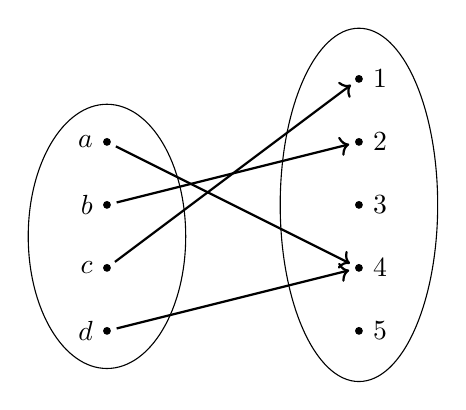
\begin{tikzpicture}[ele/.style={fill=black,circle,minimum width=.8pt,inner sep=1pt},every fit/.style={ellipse,draw,inner sep=-2pt}, scale = 0.8]
  \node[ele,label=left:$a$] (a1) at (0,4) {};    
  \node[ele,label=left:$b$] (a2) at (0,3) {};    
  \node[ele,label=left:$c$] (a3) at (0,2) {};
  \node[ele,label=left:$d$] (a4) at (0,1) {};

  \node[ele,,label=right:$1$] (b1) at (4,5) {};
  \node[ele,,label=right:$2$] (b2) at (4,4) {};
  \node[ele,,label=right:$3$] (b3) at (4,3) {};
  \node[ele,,label=right:$4$] (b4) at (4,2) {};
  \node[ele,,label=right:$5$] (b5) at (4,1) {};  
  

  \node[draw,fit= (a1) (a2) (a3) (a4),minimum width=2cm] {} ;
  \node[draw,fit= (b1) (b2) (b3) (b4) (b5),minimum width=2cm] {} ;  
  \draw[->,thick,shorten <=2pt,shorten >=2pt] (a1) -- (b4);
  \draw[->,thick,shorten <=2pt,shorten >=2] (a2) -- (b2);
  \draw[->,thick,shorten <=2pt,shorten >=2] (a3) -- (b1);
  \draw[->,thick,shorten <=2pt,shorten >=2] (a4) -- (b4);
 \end{tikzpicture}
 \caption{Eine Funktion mit einer endlichen Definitionsmenge $\mathbb{D} = \{a, b, c, d\}$  (links), einer endlichen Zielmenge $Z = \{1, 2, 3, 4, 5\}$ (rechts) und einer Bildmenge $\mathbb{W} = \{1,2,4\}$. Alle Elemente aus $\mathbb{D}$ besitzen genau eine \glqq Verbindung\grqq .}
\end{figure}

\paragraph{Beispiele:}
\begin{itemize}
\item $\mathbb{D}\rightarrow\mathbb{W}, f(x) := x^2$ bzw. $x \mapsto x^2$
\item $\mathbb{D}\rightarrow\mathbb{W}, f(x) := 42x(12x-12(3x^2))$ bzw. $x \mapsto 42x(12x - 12(3x^2))$
\end{itemize}
\end{flushleft}

\subsection{Eigenschaften von Funktionen}
\subsubsection{Surjektivit"at (Bonus)}
Eine Funktion $f$ ist surjektiv (siehe Abb. \ref{fig:surjektiv}) genau dann wenn jeder Wert der Zielmenge mindestens einmal angenommen wird:
\begin{equation*}
\forall y \in Z \ \exists x \in \mathbb{D} : f(x) = y
\end{equation*}
\begin{figure}[h!]
 \centering
 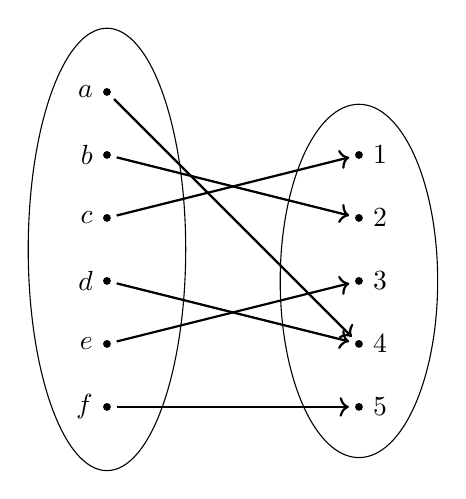
\begin{tikzpicture}[ele/.style={fill=black,circle,minimum width=.8pt,inner sep=1pt},every fit/.style={ellipse,draw,inner sep=-2pt}, scale = 0.8]
  \node[ele,label=left:$a$] (a1) at (0,6) {};    
  \node[ele,label=left:$b$] (a2) at (0,5) {};    
  \node[ele,label=left:$c$] (a3) at (0,4) {};
  \node[ele,label=left:$d$] (a4) at (0,3) {};
  \node[ele,label=left:$e$] (a5) at (0,2) {};
  \node[ele,label=left:$f$] (a6) at (0,1) {};

  \node[ele,,label=right:$1$] (b1) at (4,5) {};
  \node[ele,,label=right:$2$] (b2) at (4,4) {};
  \node[ele,,label=right:$3$] (b3) at (4,3) {};
  \node[ele,,label=right:$4$] (b4) at (4,2) {};
  \node[ele,,label=right:$5$] (b5) at (4,1) {};  
  

  \node[draw,fit= (a1) (a2) (a3) (a4) (a5) (a6),minimum width=2cm] {} ;
  \node[draw,fit= (b1) (b2) (b3) (b4) (b5),minimum width=2cm] {} ;  
  \draw[->,thick,shorten <=2pt,shorten >=2pt] (a1) -- (b4);
  \draw[->,thick,shorten <=2pt,shorten >=2] (a2) -- (b2);
  \draw[->,thick,shorten <=2pt,shorten >=2] (a3) -- (b1);
  \draw[->,thick,shorten <=2pt,shorten >=2] (a4) -- (b4);
  \draw[->,thick,shorten <=2pt,shorten >=2] (a5) -- (b3);
  \draw[->,thick,shorten <=2pt,shorten >=2] (a6) -- (b5);
 \end{tikzpicture} 
 \caption{Eine surjektive Funktion.}
 \label{fig:surjektiv}
\end{figure}

\subsubsection{Injektivit"at (Bonus)}
Eine Funktion $f$ ist injektiv (siehe Abb. \ref{fig:injektiv}) genau dann wenn jeder Wert der Bildmenge \textbf{nicht mehrmals} angenommen wird:
\begin{equation*}
\forall x_1, x_2 \in \mathbb{D} : f(x_1) = f(x_2) \Rightarrow x_1 = x_2
\end{equation*}
\begin{figure}[h!]
 \centering
 \begin{tikzpicture}[ele/.style={fill=black,circle,minimum width=.8pt,inner sep=1pt},every fit/.style={ellipse,draw,inner sep=-2pt}, scale = 0.8]
  \node[ele,label=left:$a$] (a1) at (0,4) {};    
  \node[ele,label=left:$b$] (a2) at (0,3) {};    
  \node[ele,label=left:$c$] (a3) at (0,2) {};
  \node[ele,label=left:$d$] (a4) at (0,1) {};

  \node[ele,,label=right:$1$] (b1) at (4,5) {};
  \node[ele,,label=right:$2$] (b2) at (4,4) {};
  \node[ele,,label=right:$3$] (b3) at (4,3) {};
  \node[ele,,label=right:$4$] (b4) at (4,2) {};
  \node[ele,,label=right:$5$] (b5) at (4,1) {};  
  

  \node[draw,fit= (a1) (a2) (a3) (a4) (a5) (a6),minimum width=2cm] {} ;
  \node[draw,fit= (b1) (b2) (b3) (b4) (b5),minimum width=2cm] {} ;  
  \draw[->,thick,shorten <=2pt,shorten >=2pt] (a1) -- (b1);
  \draw[->,thick,shorten <=2pt,shorten >=2] (a2) -- (b2);
  \draw[->,thick,shorten <=2pt,shorten >=2] (a3) -- (b3);
  \draw[->,thick,shorten <=2pt,shorten >=2] (a4) -- (b4);
 \end{tikzpicture} 
 \caption{Eine injektive Funktion.}
 \label{fig:injektiv}
\end{figure}

\subsubsection{Bijektion (Bonus)}
Eine Funktion ist bijektiv (siehe Abb. \ref{fig:bijectiv}), wenn sie zugleich injektiv und surjektiv ist. Eine solche Funktion ist eine eins-zu-eins Relation, sie besitzt zudem eine Umkehrfunktion.
\begin{figure}[h!]
 \centering
 \begin{tikzpicture}[ele/.style={fill=black,circle,minimum width=.8pt,inner sep=1pt},every fit/.style={ellipse,draw,inner sep=-2pt}, scale = 0.8]
  \node[ele,label=left:$a$] (a1) at (0,4) {};    
  \node[ele,label=left:$b$] (a2) at (0,3) {};    
  \node[ele,label=left:$c$] (a3) at (0,2) {};
  \node[ele,label=left:$d$] (a4) at (0,1) {};

  \node[ele,,label=right:$1$] (b1) at (4,4) {};
  \node[ele,,label=right:$2$] (b2) at (4,3) {};
  \node[ele,,label=right:$3$] (b3) at (4,2) {};
  \node[ele,,label=right:$4$] (b4) at (4,1) {};
  

  \node[draw,fit= (a1) (a2) (a3) (a4) (a5) (a6),minimum width=2cm] {} ;
  \node[draw,fit= (b1) (b2) (b3) (b4) (b5),minimum width=2cm] {} ;  
  \draw[->,thick,shorten <=2pt,shorten >=2pt] (a1) -- (b1);
  \draw[->,thick,shorten <=2pt,shorten >=2] (a2) -- (b2);
  \draw[->,thick,shorten <=2pt,shorten >=2] (a3) -- (b3);
  \draw[->,thick,shorten <=2pt,shorten >=2] (a4) -- (b4);
 \end{tikzpicture} 
 \caption{Eine bijektive Funktion.}
 \label{fig:bijectiv}
\end{figure}

\subsubsection{Umkehrfunktion}
Durch Einsetzen eines bestimmten $x$-Wertes in eine Funktion $f$ erh"alt man den entsprechenden $y$-Wert: $y=f(x)$. Will man jedoch den $x$-Wert zu einem bestimmten $y$-Wert bestimmen, so muss man zun"achst dessen Umkehrfunktion $f^{-1}$ an der Stelle $y$ berechnen: $x=f^{-1}(y)$. Daf"ur l"ost man die Gleichung $y=f(x)$ nach $x$ auf. Durch das Bilden der Umkehrfunktion werden Definitions- und Wertemenge vertauscht. Die Umkehrfunktion muss nat"urlich die Anforderungen erf"ullen welche an eine Funktion gestellt werden. Wenn nicht jedes $y$ auf genau ein $x$ abgebildet wird, existiert die Umkehrfunktion nicht. Damit muss die Funktion bijektiv sein. Ist die Funktion injektiv aber nicht surjektiv, so m"ussen wir den Definitionsbereich einschr"anken, um eine Funktion zu erhalten. 

\paragraph{Beispiel}
\begin{itemize}
\item $f(x) = x^2$ besitzt keine Umkehrfunktion denn sie ist nicht injektiv: $f(2) = f(-2) = 4$. Somit m"usste $f^{-1}(4) = \{2, -2\}$ (hier wird ein Wert $4$ der Bildmenge mehrfach angenommen) sein, was aber die Definition einer Funktion widerspricht!
\item In Abbildung \ref{fig:injektiv} m"ussten wir $5$ aus dem Definitionsbereich von $f^{-1}$ herausnehmen. Wir w"urden dann eine Umkehrfunktion erhalten, allerdings w"are $f^{-1}(5)$ nicht definiert.
\item $f(x) = e^x$ ist bijektiv falls $Z = \mathbb{R}^+  \setminus \{0\}$. F"ur $Z = \mathbb{R}$ ist sie nicht surjektiv denn $e^x$ ist stets gr"o"ser Null. Ihre Umkehrfunktion ist bekanntlich $f^{-1}(y) = \ln(y)$, diese ist aber nur auf $\mathbb{D}_{f^{-1}} =  \mathbb{R}^+ \setminus \{0\}$ definiert.
\item $f(x) = x$ ist bijektiv auf ganz $\mathbb{R}$.
\end{itemize}


\subsubsection{Monotonie}
Die Monotonie einer Funktion gibt an, ob deren Funktionswerte mit den Funktionsargumenten ansteigen oder abfallen.
\begin{itemize}
\item Eine Funktion ist \textcolor{red}{monoton fallend} \textcolor{DarkGrey}{(bzw. wachsend)}, wenn gilt:
\begin{equation*}
\forall x_1, x_2 \in\mathbb{D}, x_1 < x_2: f(x_1)\geq f(x_2) \hspace{0.2 cm}\textcolor{DarkGrey}{(bzw. f(x_1)\leq f(x_2))}
\end{equation*}
\item Eine Funktion ist \textcolor{red}{streng monoton fallend} \textcolor{DarkGrey}{(bzw. wachsend)}, wenn gilt:
\begin{equation*}
\forall x_1, x_2 \in\mathbb{D}, x_1 < x_2: f(x_1)>f(x_2) \hspace{0.2 cm}\textcolor{DarkGrey}{(bzw. f(x_1)<f(x_2))}
\end{equation*}
\end{itemize}

\subsubsection{Symmetrie} \label{sec:symmetrie}
Eine Funktion ist genau dann \textcolor{red}{symmetrisch zur y-Achse}, wenn gilt:
\begin{equation*}
f(x)=f(-x).
\end{equation*}
Solche Funktionen werden auch als \textcolor{red}{gerade} Funktion bezeichnet. Eine Funktion ist genau dann \textcolor{red}{symmetrisch zum Ursprung}, oder auch \textcolor{red}{ungerade}, wenn gilt:
\begin{equation*}
f(-x)=-f(x).
\end{equation*}
\begin{center}
\textbf{\textcolor{red}{Achtung:}} Gerade hat in dem Sinne nichts mit der Geraden zu tun!!!
\end{center}

\subsubsection{Periodizit"at}
Eine Funktion ist dann \textcolor{red}{periodisch}, wenn es eine Konstante p gibt, f"ur die gilt:
\begin{equation*}
f(x+p) = f(x), \forall x\in\mathbb{D}
\end{equation*}
Diese Definition sagt eigentlich nichts anderes aus, als dass sich die Funktion st"andig im gleichen Abstand wiederholt.

\subsubsection{Nullstellen} \label{sec:nullstellen}
Eine Nullstelle ist ein Punkt, an dem der Graph die $x$-Achse schneidet. Anders ausgedr"uckt: Ein Punkt an dem die Funktion $f(x)$ den Wert $0$ erreicht. Um Nullstellen zu berechnen, l"ost man die Gleichung
\begin{equation*}
f(x) = 0,
\end{equation*}
nach $x$. Beispiel: $f(x)=x^2-1$, Nullstellen: $x^2-1=0\implies x^2=1$, L"osungen sind $+1$ und $-1$. Die Gleichung kann also auch mehrere L"osungen haben.

\subsubsection{Stetigkeit}
Eine Funktion ist stetig, wenn man ihren Graphen (innerhalb der Definitionsmenge) ohne Absetzen des Stiftes in einem Zug zeichnen kann (salopp). Achtung folgende Definition ist eine der knackigsten Ausdr"ucke die euch begegnen wird. Eine Funktion $f : \mathbb{D} \to Z$ ist stetig in $x_0 \in \mathbb{D}$, wenn
\begin{equation*}
\forall \epsilon > 0 \ \exists \delta > 0 : \forall x \in \mathbb{D} \text{ mit } \left|x - x_0 \right| < \delta \text{ gilt: } \left| f(x) - f(x_0) \right| < \epsilon 
\end{equation*}
Intuitiv bedeutet dies: egal wie klein ich meine Funktionswert-\textbf{Umgebung} ($\epsilon$) um $f(x_0)$ w"ahle, ich kann trotzdem alle Funktionswerte, welche durch die Argument-\textit{Umgebung} ($\delta$) um $x_0$ entstehen, einschlie"sen.

\subsubsection{Verschieben einer Funktion} \label{sec:verschieben}
Angenommen wir haben eine Funktion $f$ mit $\mathbb{D} = \mathbb{R}$ und wollen eine neue Funktion $f^*$ bauen, wobei wir diese um $d > 0$ nach rechts verschieben wollen. Damit muss gelten:
\begin{equation*}
\forall x \in \mathbb{R} :  f^*(x) = f(x-d) \iff \forall x \in \mathbb{R} : f^*(x+d) = f(x).
\end{equation*}
Wir nehmen also einfach die gegebene Funktion $f(x)$ und ersetzen jedes $x$ durch $x-d$. Setzen wir hingegen $f^*(x) = f(x) + d$ so verschieben wir die Funktion nach oben. F"ur $d < 0$ folgt, dass wir die Funktion nach links bzw. nach unten verschieben.

\subsection{Lineare Funktionen}
Zu den einfachsten Funktionen geh"oren die linearen Funktionen. Alle linearen Funktionen (mit nur einer Variable) k"onnen in folgende Form gebracht werden: 
\begin{equation*}
f(x) = mx+t.
\end{equation*}
Hierbei ist $m$ der konstante Wert der Steigung:
\begin{equation*}
m= \frac{\triangle y}{\triangle x}=\frac{f(x_2)-f(x_1)}{x_2-x_1}
\end{equation*}
Die Konstante $t$ ist auch als $y$-Achsenabschnitt bekannt. Er wird so bezeichnet, da die Funktion f"ur den $x$-Wert $0$ den Funktionswert $y = t$ annimmt. Viele komplizierte Funktionen werden am Ende doch wieder mit Hilfe einfacher lineare Funktionen angen"ahert. Lineare Funktionen lassen sich auf dem Computer leicht berechnen. Sie sind so prominent und verbreitet, dass es f"ur sie eine eigenen Vorlesung gibt: \textbf{Lineare Algebra}.

%Lineare Funktionen existieren in drei Auspr"agungen. Geraden, Halbgeraden und Strecken. Eine Gerade ist unendlich lang, eine Strecke existiert nur zwischen zwei reellen Punkten und eine Halbgerade startet oder endet in genau einem Punkt. Der andere Teil geht ins Unendliche.

\subsubsection{Die Punktsteigungsform}
Um eine Gerade zu Definieren, sind immer zwei Dinge von N"oten:
\begin{itemize}
\item zwei Punkte $P_1 = (x_1, f(x_1)), P_2 = (x_2, f(x_2))$, welche auf der Geraden liegen \textbf{oder}
\item ein Punkt $P = (x_p, f(x_p))$ und die Steigung $m$ der Geraden
\end{itemize}
Im ersteren Fall berechnen wir $m$ nach obiger Gleichung $m = \frac{f(x_1) - f(x_2)}{x_1 - x_2}$ und sind im Fall 2. Um dann weiter zu verfahren, ben"otigt man die Punktsteigungsform, welche wie folgt lautet:
\begin{equation*}
f(x) = m \cdot (x-x_p) + y_p
\end{equation*}
$m$ ist hierbei wie gehabt die Steigung der Geraden und $x$ die Variable. $x_p$ und $f(x_p) = y_p$ sind jedoch die Koordinaten eines Punktes $P$, welcher auf der Geraden liegt. Nachdem man die Punktsteigungsform dann ausmultipliziert hat, besitzt man wieder die ganz normale Geradengleichung, wie oben beschrieben.

\subsubsection{Schnittpunkt zweier Geraden}
Ein Schnittpunkt zweier Funktionen ist ein Punkt, welcher sich auf beiden Graphen der Funktionen befindet. Wenn ein Punkt auf beiden Graphen sein soll, so muss er beide Funktionen erf"ullen. Seien $f_1, f_2$ Geradenfunktionen so scheiden sich die von ihnen definierten Geraden im Punkt $S = (x, y)$ wenn
\begin{equation*}
f_1(x) = f_2(x) = y
\end{equation*}

\paragraph{Beispiel:}
Nehmen wir als Beispiel die Funktionen $f_1(x) = 4x$ und $f_2(x) = 12x - 23$. Es muss nun gelten 
\begin{equation*}
	f_1(x) = f_2(x) \iff 4x = 12x - 23 \iff -8x = -23 \iff x = \frac{23}{8}
\end{equation*}
Nun muss man den erhaltenen $x$-Wert nur noch in eine der beiden Gleichungen einsetzen und man erh"alt das Ergebnis oder wir schreiben frech
\begin{equation*}
S = \left( \frac{23}{8}, f_1(23/8) \right) = \left(\frac{23}{8}, \frac{23}{2} \right)
\end{equation*}
Der Schnittpunkt hat somit die Koordinaten $S = \left(\frac{23}{8}, \frac{23}{2} \right)$.

\subsubsection{Besondere Geraden}
\begin{itemize}
\item Besitzen zwei Geraden dieselbe Steigung, so sind diese parallel zueinander. Im Normalfall besitzen diese keinerlei Schnittpunkte. Eine besondere Art der Parallelit"at ist jedoch die Identit"at zweier Geraden. Identische Geraden besitzen logischer Weise unendlich viele Schnittpunkte.
\item Sind zwei Geraden senkrecht (im rechten Winkel) zueinander, so ist das Produkt ihrer Steigungen -1: $m_1 \cdot m_2 = -1$.
\item Eine  \textcolor{red}{Tangente} ber"uhrt eine Kurve lediglich in einem einzigen Punkt.
\item Eine  \textcolor{red}{Sekante} schneidet eine Kurve in zwei Punkten.
\end{itemize}

\subsection{Quadratische Funktionen}
Nach den linearen sind die sogenannten quadratischen Funktionen noch relativ einfach. Sie werden auch als Parabelgleichungen bezeichnet. Ihren Namen verdanken diese Funktionen der Tatsache, dass ihre Variable zumindest einmal quadratisch und niemals mit einem h"oheren Exponenten als $2$ in die Funktion mit eingeht.\\
Um diese Definition jedoch richtig zu verstehen, m"ussen wir zun"achst einmal anschauen, was ein Exponent ist:

\subsection{Exponent und Basis}
Die Worte Exponent und Basis, spielen immer dann eine Rolle in der Mathematik, wenn es sich um ein Konstrukt wie $a^b$ handelt (Gesprochen: "'a hoch b"').\\
In diesem Konstrukt wird "'a"' als Basis und "'b"' als Exponent bezeichnet. Hierbei gilt:
\begin{itemize}
	\item $a^0 = 1$
	\item $a^1 = a$
	\item $a^2 = a \cdot a$
	\item $a^3 = a \cdot a \cdot a$
	\item $a^4 = a \cdot a \cdot a \cdot a$
	\item $\ldots$
\end{itemize}

\paragraph{Rechengesetze f"ur Exponenten}
\begin{enumerate}
	\item $((b)^n)^m = b^{n \cdot m}$
	\item $b^n \cdot b^m = b^{n+m}$
	\item $\frac{b^n}{b^m} = b^{n-m}$
\end{enumerate}

\noindent Will man nun, solch eine Funktion umkehren, so muss man die n-te Wurzel ziehen:
\paragraph{Beispiel f"ur Wurzeln}
\begin{enumerate}
	\item $f(x)=x^2 => f^{-1}(y)=\sqrt[2]{y}$ oder k"urzer $f^{-1}(y)=\sqrt{y}$
	\item $f(x)=x^3 => f^{-1}(y)=\sqrt[3]{y}$
	\item $f(x)=x^4 => f^{-1}(y)=\sqrt[4]{y}$
\end{enumerate}

\paragraph{Rechengesetze f"ur Wurzeln}
\begin{enumerate}
	\item $\sqrt[m]{a} = a^{\frac{1}{m}}$
	\item $\sqrt[m]{a} \cdot \sqrt[m]{b} = \sqrt[m]{a \cdot b}$
	\item $\frac{\sqrt[m]{a}}{\sqrt[m]{b}} = \sqrt[m]{\frac{a}{b}}$
	\item $\sqrt[m]{b^n} = b^{\frac{n}{m}}$
\end{enumerate}\vline

\noindent Im Fall $a^2$ wird auch oft einfach nur "'a zum Quadrat"' gesagt.\\
Dies kommt daher, dass ein Quadrat aus vier gleich langen Seiten besteht und es sich bei allen Innenwinkel (die Winkel innerhalb des Rechtecks), um so genannte "'rechte Winkel"' (genau 90 Grad) handelt. Die Fläche eines Quadrats, mit der Seitenl"ange a, l"asst sich deshalb mit der Formel $a \cdot a$ oder auch $a^2$ berechnen.

\subsubsection{Die Normalparabel}
Die Normalparabel besitzt die Formel 
\begin{equation*}
f(x) = x^2
\end{equation*}
Sie ist eine nach oben ge"offnete, achsensymmetrische Kurve dar, deren niedrigster Punkt (Scheitel) $S$ im Ursprung des Koordinatensystems $(0,0)$ liegt.

%Siehe: Verschieben einer Funktion
%\subsubsection{Verschieben einer Parabel}
%Wollen wir eine 
%Eine Parabel l"asst sich um den Wert $x_s$ in $x$-Richtung verschieben, indem man diesen Wert von der Variable $x$ subtrahiert, daraus folgt:\\
%$f(x)=(x-x_s)^2$\vspace{0.25 cm}\flushleft
%Durch Addition des gesamten Terms mit dem Wert $y_s$ wird die Parabel um den gleichen Wert in y-Richtung verschoben.\\
%Die Gleichung der Parabel lautet nun wie folgt:\\
%$f(x)=(x-x_s)^2+y_s$\\
%Ihr Scheitel besitzt die Koordinaten $S(x_s,y_s)$.

\subsubsection{Stauchen und Strecken}
Durch Multiplizieren der Normalparabel mit einer konstanten $a$ l"asst sich die Kurve stauchen oder strecken $f(x)=a \cdot x^2$. Ist der Betrag von $a$ kleiner $1$, so wird die Parabel gestaucht (siehe Abb. \ref{fig:parabel}). Ist er gr"o"ser $1$, so wird sie gestreckt. Dar"uber hinaus wird die Funktion durch einen negativen Wert von a an der $x$-Achse gespiegelt und die Parabel ist somit nach unten ge"offnet.
\begin{figure}[h!]
\begin{center}
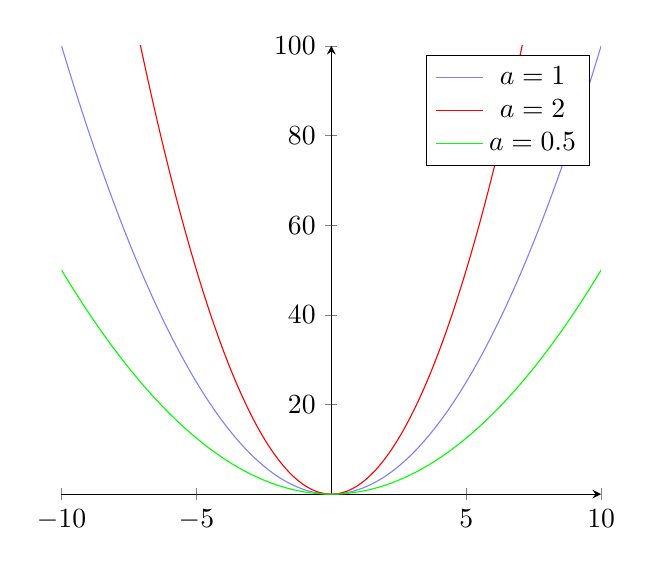
\begin{tikzpicture}[scale = 1.0]
    \begin{axis}[
        domain=-10:10,
        xmin=-10, xmax=10,
        ymin=-0, ymax=100,
        samples=400,
        axis y line=center,
        axis x line=middle,
    ]
    	  \addlegendentry{$a=1$}
    	   \addplot+[mark=none, color=blue] {x*x};
    	   \addlegendentry{$a=2$}
       \addplot+[mark=none, color=red] {2 * x*x};
       \addlegendentry{$a=0.5$}
       \addplot+[mark=none, color=green] {0.5 * x*x};
    \end{axis}
\end{tikzpicture}
\end{center}
\caption{Normalparabel (blau), gestreckte (rot) und gestauchte Normalparabel (gr"un).}
\label{fig:parabel}
\end{figure}

\subsubsection{Die Scheitelform}
Durch Kombination von Stauchung/Streckung und Verschiebung erh"alt man die so genannte Scheitelform: 
\begin{equation*}
f(x)=a(x-x_s)^2+y_s.
\end{equation*}
Mithilfe dieser Form lassen sich alle Arten quadratischer Funktionen darstellen. Au"serdem lassen sich die Koordinaten des Scheitels, der Stauchungs- bzw. Streckungsfaktor der Funktion, sowie die Frage, ob sie nach oben oder unten ge"offnet ist, auf einfachste Weise bestimmen.

\subsubsection{Die Normalform einer quadratischen Gleichung}
Multipliziert man die Scheitelform aus, so erh"alt man 
\begin{equation*}
f(x)=a \cdot x^2-2 \cdot a \cdot x_sx+x_s^2+y_s.
\end{equation*}
Ersetzt man nun die konstanten Werte $-2ax_s$ durch $b$ und $x_s^2+y_s$ durch $c$, so erh"alt man die \textbf{Normalform} quadratischer Gleichungen:
\begin{equation*}
f(x)=a \cdot x^2+b \cdot x+c
\end{equation*}

\subsubsection{Die binomischen Formeln}
Die binomischen Formeln sind das Ergebnis des Ausmultiplizierens, hat man sie jedoch im Kopf so spart man viel Zeit:
\begin{enumerate}
\item $(a+b)^2=a^2+2ab+b^2$
\item $(a-b)^2=a^2-2ab+b^2$
\item $(a+b)(a-b)=a^2-b^2$
\end{enumerate}

\subsubsection{Die quadratische Erg"anzung}
Die quadratische Erg"anzung hilft uns bei der Umwandlung der Normalform in die Scheitelform und somit bei der Bestimmung des Scheitels. Wir werden diese an anhand eines Beispiels erkl"aren.

\paragraph{Beispiel:}
Sei 
\begin{equation*}
f(x) = 3x^2 - 6x - 24.
\end{equation*}
Im ersten Schritt klammern wir die Konstante "'$a$"' (hier gleich $3$) aus:
\begin{equation*}
f(x) = 3x^2 - 6x - 24= 3 \cdot (x^2-2x-8).
\end{equation*}
Schaut man sich nun den Term innerhalb der runden Klammern genauer an, so kann man eine gewisse "Ahnlichkeit mit der ersten, bzw. zweiten binomischen Formel feststellen. Deshalb folgt nun auch der wichtigste Schritt, die eigentliche quadratische Erg"anzung. Wir erg"anzen die Formel nun so, dass wir eine der beiden binomischen Formeln anwenden k"onnen. Daf"ur m"ussen wir erst einmal feststellen, was der $a$- und was der $b$-Wert der binomischen Formeln ist. Die zweite binomische Formel lautet 
\begin{equation*}
(a-b)^2=a^2-2ab+b^2.
\end{equation*}
Vergleichen wir dies mit unserem Term 
\begin{equation*}
x^2-2x-8
\end{equation*}
so sehen wir gleich, dass
\begin{equation*}
a := x \Rightarrow 2ab = 2x \Rightarrow b = 1.
\end{equation*}
Allerdings ist $b^2$ f"ur $b = +1$ nicht $-8$ sondern $1$. Um $f$ nicht zu ver"andern m"ussen wir deshalb eine Korrektur vornehmen:
\begin{equation*}
f(x) = 3 \cdot \left(  \underbrace{(x-1)^2}_{\text{wegen 2. bin. Formel}} + \underbrace{-1^2 - 8}_{\text{da } b^2 = 1 \text{ und nicht } -8 } \right)
\end{equation*}
Hier nochmal die "Ubersicht:
\begin{equation*}
f(x) = 3 \cdot \left(  \underbrace{x^2}_{:=a^2} \underbrace{- 2 \cdot x \cdot 1}_{:= -2ab} \underbrace{+ 1^2}_{:= + b^2} \underbrace{- 1^2 -8}_{:=-\text{Korrektur}} \right)
\end{equation*} 
Nun k"onnen wir noch ein wenig zusammenfassen
\begin{equation*}
f(x) = 3 \cdot ((x-1)^2-1^2-8) = 3((x-1)^2-9) = 3(x-1)^2-27
\end{equation*}
Und voil\`a, schon ist man fertig.

\subsubsection{Berechnung der Nullstellen} \label{sec:quadnullstellen}
Um die Nullstellen von quadratischen Gleichungen zu berechnen, gibt es mehrere M"oglichkeiten.

\paragraph{Zerlegung in Linearfaktoren (auch f"ur Polynome):}
%\begin{center}
%"'Null multipliziert mit irgendwas ist immer Null"'
%\end{center} % Bitte entfernen. Unendlich mal Null ist undefiniert, und gerade bei Grenzwerten schwierig...

Mit der Linearfaktorzerlegung erhalten wir eine Form der Funktion, die uns sagt f"ur welche $x$ ein Faktor Null und somit die gesamte Funktion Null ergibt. Auch dies zeigen wir an einem Beispiel.

\paragraph{Beispiel}
Sei
\begin{equation*}
f(x) = 6x^2 - 24
\end{equation*}
Wir fragen uns f"ur welche $x$ ist $f(x) = 0$.
\begin{equation*}
f(x) = 0 \iff 6x^2 - 24 = 0 \iff x^2 - 4 = 0 \stackrel{\text{3. bin. Formel}}{\iff} (x-2)(x+2) = 0 
\end{equation*}
Die Faktoren der Funktion sind somit $(x-2)$ und $(x+2)$. $(x-2) = 0$ f"ur $x = 2$ und $(x+2) = 0$ f"ur  $x = -2$. Damit sind die Nullstellen:
\begin{equation*}
N_1 = (2, f(2)) = (2, 0) \text{ und } N_2 = (-2, f(-2)) = (-2, 0)
\end{equation*}

\paragraph{Berechnung der Umkehrfunktionen (f"ur alle Funktionen):}
Im Grundlagenteil haben wir den Begriff der Umkehrfunktion kennen gelernt. Angenommen $x_0$ sei eine Nullstelle der Funktion $f(x)$ und angenommen $f(x)$ besitzt eine Umkehrfunktion ($f(x)$ ist bijektiv), dann folgt daraus:
\begin{equation*}
f(x_0) = 0 \iff f^{-1}(0) = x_0
\end{equation*}
Das hei"st wir k"onnten $f^{-1}(x)$ berechnen und dann einfach $0$ einsetzten und erhalten damit die Nullstelle von $f(x)$ nämlich $N = (f^{-1}(0), 0)$.

\paragraph{Beispiele}
\begin{itemize}
\item Sei $f(x) = 3x^2 + 3x + 4$, $f$ ist nicht bijektiv, hier nehmen wir lieber die Mitternachtsformel.
\item Sei $f(x) = x - 7 \Rightarrow f^{-1}(y) = y + 7 \Rightarrow N = (f^{-1}(0), 0) = (7, 0)$.
\item Sei $f(x) = \ln(x)$, die Umkehrfunktion ist $e^x$ und somit ist $e^0 = 1$ eine Nullstelle von $f(x)$.
\end{itemize}

% Was hier folgt ist unsinnig!
%Wenn wir also rein theoretisch die Funktion umkehren und 0 einsetzen, so m"ussten wir die x-Werte der Nullstellen herausbekommen. Wollen wir jedoch eine quadratische Gleichung umkehren, so sto"sen wir allerdings auf ein kleines Problem... \vspace{0.5 cm}\\
%Schauen wir uns daf"ur mal ein Beispiel an:\\
%$y = $\\
%Zun"achst m"usste man daf"ur sorgen, dass das x nicht mehr in zwei verschiedenen Potenzen auftaucht. Dies geht ganz leicht "uber die quadratische Erg"anzung.\\
%$y = 3(x + 0,5)^2 + 3,25 | -3,25\leftrightarrow$\\
%$3(x+0,5)^2 = y-3,25 | :3 \leftrightarrow$\\
%$(x+0,5)^2 = \frac{y-3,25}{3}$\\
%Nun m"ussten wir die Wurzel ziehen. Hier kommt das Problem zum Vorschein.\\
%Die Wurzel einer bestimmten Zahl kann sowohl positiv als auch negativ sein.\\
%Nehmen wir zum Beispiel die Zahl 4: ihre Wurzel ist $\pm 2$.\\
%Da die Regel, dass jedem x-Wert genau ein y-Wert zugeordnet wird, nicht mehr erf"ullt wird, handelt es sich nicht mehr um eine Funktion, sondern um eine Relation.
%Aus diesem Grund gilt auch f"ur unsere Gleichung:\\
%$x+0,5 =\pm \sqrt{\frac{y-3,25}{3}}\leftrightarrow$\\
%$x=0,5 \pm \sqrt{\frac{y-3,25}{3}}$\\
%Nun muss man noch f"ur y  0 einsetzen und gucken was passiert.\\
%In unserem Fall bemerkt man schnell, dass unter der Wurzel ein negativer Wert heraus kommt. Dies darf jedoch nicht sein, da in den reellen Zahlen die Wurzel von negativen Zahlen nicht definiert ist.\\
%Somit hat unsere Funktion keinerlei Nullstellen.

\paragraph{Die L"osungsformel f"ur quadratische Gleichungen (Mitternachtsformel):}
Eine weitere M"oglichkeit, die Nullstellen einer quadratischen Funktion zu berechnen, w"are durch Verwendung der so genannten "'Mitternachtsformel"':
\begin{equation*}
0 = ax^2 + bx + c \Rightarrow x_{1,2} := \frac{-b \pm \sqrt{b^2 - 4ac}}{2a}
\end{equation*}
Falls jedoch 
\begin{equation*}
b^2 - 4ac < 0
\end{equation*}
existiert \textbf{keine Nullstelle}, da wir in den reellen Zahlen keine negative Wurzel kennen und falls
\begin{equation*}
b^2 - 4ac = 0
\end{equation*}
handelt es sich um eine sog. \textbf{doppelte Nullstelle}. Ansonsten handelt es sich um \textbf{zwei Nullstellen}. Dabei nennen wir $b^2 - 4ac$ die Diskriminante.
%Wie man sieht, ist es sehr umst"andlich, jedes Mal die Umkehrrelation zu berechnen und in diese dann f"ur y den Wert 0 einzusetzen... Aus diesem Grund wurden allgemeine Formeln zur Berechnung der Nullstellen quadratischer Gleichungen hergeleitet:\\
%Zun"achst hat man die allgemeine Formel $y = ax^2 + bx +c$ gegeben.\\
%Diese wird "'gleich Null"' gesetzt:\\
%$0 = ax^2 + bx + c$\\
Wie entsteht diese Formel?
\begin{equation*}
 ax^2 + bx + c 
\end{equation*}
Wird auf die Scheitelform gebracht
\begin{equation*}
 ax^2 + bx + c  = \left(x + \frac{b}{2a} \right)^2 - \frac{b^2-4ac}{4a^2}
\end{equation*}
und gleich Null gesetzt
\begin{equation*}
\left(x + \frac{b}{2a}\right)^2 - \frac{b^2-4ac}{4a^2} = 0 \iff x = \frac{-b \pm \sqrt{b^2 - 4ac}}{2a}
\end{equation*}
Den Beinamen "'Mitternachtsformel"' verdankt sie ihrer Wichtigkeit. Sie wird n"amlich tats"achlich so oft gebraucht, dass man sie auch noch auswendig aufsagen k"onnen sollte, wenn man um Mitternacht gefragt wird!% (Auch wenn von euch vermutlich niemand bereits um Mitternacht schl"aft $\ldots$).

\paragraph{Raten der Nullstellen (f"ur alle Funktionen):}
Ist man erfahren genug und die Funktion einfach genug, so kann man h"aufig die Nullstelle auch einfach erraten. Dann muss man noch einen Beweis erbringen, dass es sich wirklich um einen Nullstelle handelt. Hierf"ur setzten wir einfach das geratene $x_0$ in $f(x)$ ein und "uberpr"ufen ob 
\begin{equation*}
f(x_0) \stackrel{?}{=} 0
\end{equation*}

%\begin{description}
%\item[Zwei Nullstellen] Die Funktion besitzt zwei Nullstellen, wenn der Wert der Diskriminante gr"o"ser 0 ist.
%\item[Eine Nullstelle] Die Funktion besitzt nur eine (doppelte) Nullstelle, wenn die Diskriminante 0 ergibt.
%\item[Keine Nullstelle] Die Funktion hat keinerlei Nullstellen, wenn f"ur die Diskriminante ein Wert kleiner 0 heraus kommt.
%\end{description}

\subsection{"Ubungen}
\begin{enumerate}
\item Berechnen Sie die Scheitelpunkte folgender Gleichungen
\begin{itemize}
\item $f(x) = 3x^2 - 3x + 6$
\item $f(x) = x^2 - 8x - 4$
\item $f(x) = x^2 + 4x + 1$
\item $f(x) = -4x^2 + 16x - 1$
\end{itemize}
\item Berechnen Sie die Nullstellen der oberen Gleichungen
\end{enumerate}

\subsection{Polynome} \label{polynom}
\subsubsection{Was ist ein Polynom}
Bei Funktionen der Form $f(x) = a_n x^b + a_{n-1} x^{b-1} + a_{n-2} x^{b-2} + ... a_0$ handelt es sich um so genannte Polynome. Da sie sehr einfach differenzierbar und integrierbar sind, haben sie eine sehr wichtige Rolle als mathematisches Werkzeug, vor allem in der Numerik. Hier nähert man komplexe Funktionen mit Polynomen an und kann diese dann einfach ableiten oder integrieren, was mit der komplexen Funktion meist nicht so einfach ist.

\subsubsection{Nullstellenberechnung mithilfe der Polynomdivision (Bonus)}
Im Folgenden werde wir nun anhand des Beispiels 
\begin{equation*}
f(x) = 6x^3 - 12x^2 - 6x + 12
\end{equation*}
die Nullstellenberechnung mithilfe der Polynomdivision erläutern. Dabei werden alle Nullstellen erraten. Jede Nullstelle liefert einen Linearfaktor. 
\begin{enumerate}
\item Wie immer setzen wir die Funktion gleich Null und werden den Faktor los:
\begin{equation*}
6x^3 - 12x^2 - 6x + 12 = 0 \iff x^3 -2x^2 - x + 2 = 0
\end{equation*}

\item Nun muss man (leider) die erste Nullstelle "'erraten"'. Da es aber sehr viele Zahlen gibt, würde dies ohne einen kleinen Trick sehr schwer werden. Besitzt ein Polynom lediglich ganzzahlige Koeffizienten, so sind die $x$-Werte der Nullstellen ganzzahlige Teiler von des letzten Koeffizienten ($a_0$). Warum dies so ist, schauen wir uns später an. Unser Beispiel kann also nur Nullstellen bei $x$-Werten aus $\{-1, 1, -2, 2\}$, besitzen. Nun kann man systematisch alle möglichen Kandidaten abarbeiten oder sieht es direkt. Testen mit $x \stackrel{?}{=} -1$:
\begin{equation*}
(-1)^3 - 2(-1)^2 - (-1) + 2 = 0
\end{equation*}
Glücklicherweise haben wir schon beim ersten Versuch eine Nullstelle bei $x_1 = -1$ entdeckt.
\item Nun werden wir uns die Eigenschaft des Faktorisierens zu Nutze machen, dass jedes Polynom in Faktoren $(x-x_{Nullstelle})$ zerlegt werden kann. Wir werden nun eine Division des Polynoms durch $(x-(-1)) = (x + 1)$ durchführen:
\polylongdiv{x^3 -2x^2 - x + 2}{x + 1}

\item Jetzt beginnt der Vorgang mit der neuen Funktion ($g(x) = x^2 - 3x + 2$), welche einen Grad weniger hat von Neuem. In unserem Fall jedoch, da wir nun eine quadratische Funktion haben, können wir die Mitternachtsformel zur Lösung heranziehen. Die drei Nullstellen unserer Beispielfunktion lauten:
\begin{equation*}
x_0 = -1; x_1 = 1; x_2 = 2
\end{equation*}
Die Funktion lässt sich also auch wie folgt schreiben:
\begin{equation*}
f(x)=(x+1)(x-1)(x-2)
\end{equation*}
\end{enumerate}
Anhand der "'neuen Darstellungsart"' der Funktion können wir sehen, warum alle Nullstellen, unter der Voraussetzung, dass sie alle ganzzahlig sind, ganzzahlige Teiler des letzten Koeffizienten sind.\\
Nehmen wir dafür ein generisches Beispiel zur Hand:\\
$f(x)=(x-a)(x-b)(x-c)=(x^2 - ax - bx + ab)(x-c)=(x^3 - ax^2 - bx^2 + abx - cx^2 + acx + bcx - abc)$\\
Man kann also sehen, dass der Betrag des letzten Koeffizienten lediglich die Multiplikation aller Nullstellen ist. Sind diese nun alle ganzzahlig, so ist auch jede Nullstelle ein ganzzahliger Teiler des letzten Koeffizienten.

\subsection{Übungen}
Berechne die Nullstellen folgender Gleichungen:
\begin{itemize}
\item $f(x) = x^4 - 2x^2 + 1$
\item $f(x) = 3x^3 + 12x^2 + 3x - 18$
\end{itemize}

\subsubsection{Rechnen mit Exponenten}
Wie ihr vielleicht schon bemerkt habt, gibt es bei den \textcolor{red}{geometrischen Folgen} eine neue mathematische Schreibweise ($q^n$). Die Konstante $q$ wird hierbei als \textcolor{red}{Basis} bezeichnet, während $n$ \textcolor{red}{Exponent} genannt wird. Hierbei gilt:
\begin{itemize}
\item $q^0 = 1$
\item $q^1 = q$
\item $q^2 = q \cdot q$
\item $q^3 = q \cdot q \cdot q$
\item $q^4 = q \cdot q \cdot q \cdot q$
\item $\ldots$
\end{itemize}

\paragraph{Rechengesetze für Exponenten}
\begin{enumerate}
\item $((b)^n)^m = b^{n \cdot m}$
\item $b^n \cdot b^m = b^{n+m}$
\item $\frac{b^n}{b^m} = b^{n-m}$
\end{enumerate}

\paragraph{Rechengesetze für Wurzeln}
\begin{enumerate}
\item $\sqrt[m]{a} = a^{\frac{1}{m}}$
\item $\sqrt[m]{a} \cdot \sqrt[m]{b} = \sqrt[m]{a \cdot b}$
\item $\frac{\sqrt[m]{a}}{\sqrt[m]{b}} = \sqrt[m]{\frac{a}{b}}$
\item $\sqrt[m]{b^n} = b^{\frac{n}{m}}$
\end{enumerate}

\subsection{Trigonometrische Funktionen}
\subsubsection{Die Winkelfunktionen rechtwinkliger Dreiecke}
Grundlegend gibt es drei Winkelfunktionen, welche auf rechtwinklige Dreiecke angewandt werden k"onnen:
\begin{itemize}
\item Sinus $\sin : \mathbb{R} \to \mathbb{R}, \mathbb{W} = \left[-1;1 \right]$
\item Kosinus $\cos : \mathbb{R} \to \mathbb{R}, \mathbb{W} = \left[ -1;1 \right]$
\item Tangens $\tan : \left( \mathbb{R} \setminus \left\{ k \pi + \frac{\pi}{2}, k \in \mathbb{Z} \right\} \right) \to \mathbb{R}, \mathbb{W} = \mathbb{R}$
\end{itemize}
\begin{warning}
	Der Tangens ist f"ur die Nullstellen des Kosinus nicht definiert denn
	\begin{equation*}
	\tan(x) := \frac{\sin(x)}{\cos(x)}
	\end{equation*}
\end{warning}
Die drei Seiten des Dreiecks werden als Hypotenuse (l"angste Seite des Dreiecks, -gegen"uber des rechten Winkels-), Ankathete (kurze Seite, welche am Winkel $\alpha$ anliegt), und Gegenkathete (Seite gegen"uber des Winkels $\alpha$) bezeichnet.
\begin{minipage}{0.45\textwidth}
\hfill
\begin{enumerate}
\item $\sin(\alpha)=\frac{\text{Gegekathete}}{\text{Hypotenuse}}$
\item $\cos(\alpha)=\frac{\text{Ankathete}}{\text{Hypotenuse}}$
\item $\tan(\alpha)=\frac{\sin(\alpha)}{\cos(\alpha)}= \frac{\text{Gegenkathete}}{\text{Ankathete}}$
\end{enumerate}
\end{minipage}
\begin{minipage}{0.45\textwidth}
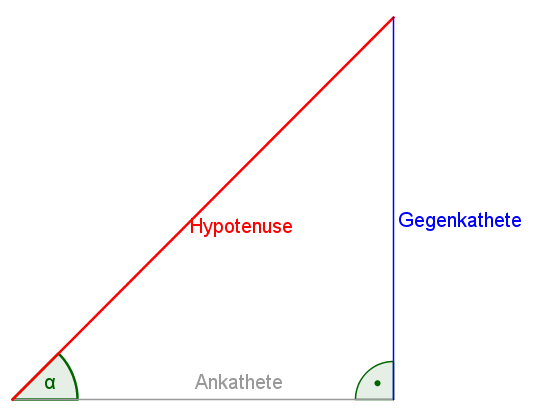
\includegraphics[width=1.0\textwidth]{pictures/TrigonDreieck}
\end{minipage}

\subsubsection{Der Einheitskreis}
Am besten sieht man die Eigenschaften der Winkelfunktionen bei der Betrachtung des \textcolor{red}{Einheitskreises}. Der Einheitskreis ist an sich nichts anderes als ein Kreis, mit Radius $r$ = 1 LE (L"angeneinheiten) und Kreismittelpunkt im Ursprung. Dabei ist die $x$-Koordinate des Punktes, am Ende der Hypotenuse des eingezeichneten Dreiecks, der Kosinuswert des Winkels Alpha und die $y$-Koordinate der Sinuswert. Der Tangens ist die Steigung der Hypotenuse. Der Zusammenhang zwischen Einheitskreis und den Funktionen ist in Abb. \ref{fig:circ} zu sehen.

\begin{figure}[h!]

\begin{tikzpicture}
% Axis
\draw[thick,-stealth,black] (-3,0)--(4,0) coordinate (A) node[below] {$x$}; % x axis
\draw[thick,-stealth,black] (0,-3)--(0,3) node[left] {$y$}; % y axis
\draw[black,thin] (0,0) circle (2.5cm);
\node[black,below] at (2.7,0) {1};
\node[black,above] at (0.2,-3.2) {1};

\draw[ultra thick,orange] (0,0) -- (\theangle:2.5cm |- 0,0) node[midway,above] {$\cos(\alpha)$}; % UpOn y axis

\draw (1,0) arc (0:\theangle:1) node at ($(\theangle/2:0.7)$) {$\alpha$};
\draw[dashed, cyan] (\theangle:2.5cm) -- (\theangle:2.5cm |- 0,0) node[sloped, rotate=180, yshift=8pt, midway] {$\sin(\alpha)$}; % vertical line
\draw[ultra thick,red,rotate=\theangle] (0,0) -- (2.5,0) coordinate (B); 

\draw[dashed,red] (0,0) -- (-2.5,-2.097);

\draw[ultra thick, blue] (-2.5,0) -- (-2.5,-2.097) node[sloped, midway,below] {$\tan(\alpha)$};;

\foreach \x in {0,30,...,360} {\filldraw[black] (\x:2.5cm) circle(1pt);};
\foreach \x/\xtext in {
        30/\frac{\pi}{6},
        60/\frac{\pi}{3},
        120/\frac{2\pi}{3},
        150/\frac{5\pi}{6},
        210/\frac{7\pi}{6},
        240/\frac{4\pi}{3},
        300/\frac{5\pi}{3},
        330/\frac{11\pi}{6}
        }
    \draw (\x:2.8cm) node {\tiny $\xtext$};
 \foreach \x/\xtext in {
        90/\frac{\pi}{2}}
        \draw (\x:2.7cm) node[xshift=4pt] {\tiny $\xtext$};    
 \foreach \x/\xtext in {
        270/\frac{3\pi}{2}}
        \draw (\x:2.7cm) node[xshift=-5pt] {\tiny $\xtext$};  
 \foreach \x/\xtext in {
        180/\pi,
        360/2\pi}
        \draw (\x:2.7cm) node[yshift=4pt] {\tiny $\xtext$};             

\begin{scope}
\begin{axis}[
    thick,
    y=2.5cm,
    axis lines=center,
    xmin=0, xmax=360,
    ymin=-1, ymax=1,
    anchor=origin, at=(A),
    xshift=3ex,
    enlarge y limits,
    enlarge x limits=upper,
    samples=90,
    xtick={0,30,...,360},
xticklabels={0,
    $\frac{\pi}{6}$,
    $\frac{\pi}{3}$,
    $\frac{\pi}{2}$,        
    $\frac{2\pi}{3}$,
    $\frac{5\pi}{6}$,
    $\pi$,
    $\frac{7\pi}{6}$,
    $\frac{4\pi}{3}$,
    $\frac{3\pi}{2}$,        
    $\frac{5\pi}{3}$,
    $\frac{11\pi}{6}$,
    $2\pi$
    },
    tick label style={font=\tiny},
    ]
    \addplot[domain=0:\theangle,ultra thick, no markers,cyan] {sin(x)} coordinate (C);
    \addplot[domain=\theangle-1:\theangle,ultra thick, no markers,cyan] {sin(x)-sin(x)} coordinate (K);

\end{axis}
\draw [dashed,red, thick] (B) -- (C);
\draw [dashed,cyan, thick] (C) -- (K);
\end{scope}
\tkzDrawPoints(B);
\end{tikzpicture}
\caption{Einheitskreis (links) und die Sinusfunktion (rechts).}
\label{fig:circ}
\end{figure}

\subsubsection{Winkelma"s und Bogenma"s}
Bisher haben wir immer mit Winkelma"sen gerechnet, wie zum Beispiel $\alpha = 45^\circ$. Neben dieser M"oglichkeit, Winkel auszudr"ucken, gibt es auch noch das Bogenma"s $b = 2\pi \ rad$. Das Bogenma"s ist die L"ange des Kreisbogens mit dem Radius $r = 1$ unter einem bestimmten Winkel. Die Umrechnung ist einfach
\begin{equation*}
rad(\alpha) = 2\pi \frac{\alpha}{360} rad \text{ f"ur } \alpha \in \left[ 0^\circ;360^\circ \right] \quad rad^{-1}(b) = 360 \cdot {\frac{b}{2\pi}}^\circ \text{ f"ur } b \in \left[0;2\pi\right]
\end{equation*}
Wie ein Winkelwert mit $^\circ$ gekennzeichnet wird, so kennzeichnet man das Bogenma"s mit dem W"ortchen "'$rad$"'.
\begin{warning}
	An den meisten "'h"oheren"' Schulen wird das Bogenma"s bevorzugt.\\
	Ihr solltet eure Taschenrechner dementsprechend umstellen (meist ist dies "uber eine \textit{Mode}-Taste zu bewerkstelligen)
\end{warning}

\begin{figure}[h!]
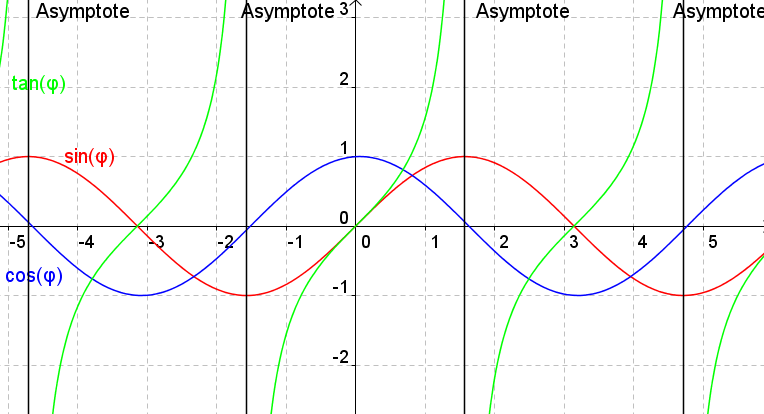
\includegraphics[width = 13 cm, height = 5 cm]{pictures/Winkelfunktionen}
\caption{Funktionsgraphen von Sinus, Kosinus und Tangens}
\end{figure}

\subsubsection{Nullstellen, Asymptoten und Symmetrie}
Alle Winkelfunktionen sind periodisch. Deshalb treten auch ihre Nullstellen in gleichbleibenden Abst"anden auf.
\begin{itemize}
\item Sinusfunktion:
\begin{equation*}
 \sin(x) = 0 \iff x \in \left\{ k \pi, k \in \mathbb{Z} \right\},
\end{equation*}
was sich mit den Nullstellen des Tangens deckt.
\item Kosinusfunktion: 
\begin{equation*}
 \cos(x) = 0 \iff x \in \left\{ k \pi + \frac{\pi}{2}, k \in \mathbb{Z} \right\},
\end{equation*}
was sich mit den Definitionsl"ucken des Tangens deckt.
\end{itemize}
Des Weiteren besitzt die Tangensfunktion eine periodisch auftretende senkrechte Asymptote an den Nullstellen des Kosinus.
Betrachtet man die Graphen im Hinblick auf ihre Symmetrie bez"uglich des Koordinatensystems, stellt man fest, dass die Sinus- und Tangesnsfunktion \textbf{punktsymmetrisch} zum Ursprung (ungerade) und die Kosinusfunktion achsensymmetriesch zur $y$-Achse (gerade) ist.

\subsubsection{Periodizit"at}
Eine Funktion ist dann \textcolor{red}{periodisch}, wenn es eine Konstante p gibt, f"ur die gilt:
\begin{equation*}
f(x+p) = f(x), \forall x\in\mathbb{D}
\end{equation*}
Diese Definition sagt eigentlich nichts anderes aus, als dass sich die Funktion st"andig im gleichen Abstand wiederholt.


\psection{Differentiation}
Beim Ableiten m"ochten wir etwas "uber die Ver"anderung einer Funktion erfahren. Angenommen ein Auto startet an einem Punkt und die Funktion $s(t)$ gibt an wie viele Meter das Auto zum Zeitpunkt $t$ zur"uckgelegt hat. Wir fragen uns nun wie schnell das Auto nach 10 Sekunden f"ahrt. Wie k"onnen wir dies herausfinden? Wir k"onnen das absch"atzen indem wir 
\begin{equation*}
\bar{v} = \frac{\text{Strecke}}{\text{Zeit}} \approx \frac{s(11) - s(9)}{11 - 9} = \frac{\Delta s}{\Delta t} = \frac{s(11) - s(9)}{2}
\end{equation*}
Aber ist $\bar{v} \stackrel{?}{=} v(10)$? Nein $\bar{v}$ ist nur die durchschnittliche Geschwindigkeit zwischen $s(9)$ und $s(11)$. Wenn wir die Geschwindigkeit genauer bestimmen m"ochten, m"ussen wir den Abstand/die \textit{Umgebung} von/um $10$ kleiner w"ahlen, $0$ darf er jedoch nicht werden, denn wir d"urfen nicht durch Null teilen. Hilfe gibt uns der Grenzwert:
\begin{equation*}
v(10) = \lim\limits_{h \to 0} \frac{s(10+h) - s(10)}{h}
\end{equation*}
Der Grenzwert muss nat"urlich existieren! Nehmen wir einmal an das Auto beschleunigt und $s(t) = 2 t^2$.
\begin{align*}
v(10) &= \lim\limits_{h \to 0} \frac{s(10+h) - s(10)}{h} = \lim\limits_{h \to 0} \frac{2 (10+h)^2 - 2 (10)^2}{h}\\
&= \lim\limits_{h \to 0} \frac{40h + 2h^2}{h} = \lim\limits_{h \to 0}(40 + 2h) \to 40
\end{align*}

\subsection{Ableiten von Funktionen}
Die Ableitung der Funktion $f$ an der Stelle $x_0$, geschrieben $f'(x_0)$ beschreibt das Verhalten der Funktion in der \textit{Umgebung} an der Stelle $x_0$. Sie ist auch die Steigung der Funktion an dem Punkt $x_0$. Die Tangente an $x_0$ hat die Steigung $f'(x_0)$. Eine Tangente ist eine Gerade, die den Graphen in nur einem einzigen Punkt ber"uhrt. Um die Tangentensteigung zu erhalten, betrachtet man zun"achst die Steigung einer Sekante und n"ahert den zweiten Punkt dem ersten immer weiter an.
\begin{definition}[Differenzierbarkeit in $x_0$]
Eine Funktion hei"st differenzierbar an der Stelle $x_0$ wenn der Grenzwert
\begin{equation*}
 \lim\limits_{x \to x_0} \frac{f(x)-f(x_0)}{x-x_0} = \lim\limits_{h \to 0}  \frac{f(x_0 + h)-f(x_0)}{h} , \text{ mit } h = x - x_0
\end{equation*}
existiert. Dieser Grenzwert wird Ableitung nach $x$ an der Stelle $x_0$ genannt und wird als $f'(x_0)$ oder $\frac{df}{dx}(x_0)$ notiert.
\end{definition}
Ein Grenzwert $a$ an der Stelle $x_0$ der Funktion $f$ existiert wenn der linke Grenzwert gleich dem rechten Grenzwert gleich dem Funktionswert gleich $a$ ist, also
\begin{equation*}
 \lim\limits_{x \to x_0^+} \frac{f(x)-f(x_0)}{x-x_0} =  \lim\limits_{x \to x_0^-} \frac{f(x)-f(x_0)}{x-x_0} = f(x_0) = a
\end{equation*}

\begin{definition}[Differenzierbarkeit]
Eine Funktion hei"st differenzierbar, wenn sie an jeder Stelle $x_0 \in \mathbb{D}$ differenzierbar ist.
\end{definition}

\paragraph{Anmerkung:} Eine differenzierbare Funktion ist stetig und eine in $x_0$ differenzierbare Funktion ist stetig in $x_0$. Die Umkehrung gilt nicht!

\subsubsection{Die erste Ableitung}
F"ur die gew"ohnlichen differenzierbaren Funktionen gibt es die uns bekannten Ableitungsregeln. Um eine Funktion abzuleiten multipliziert man bei Polynomen jeweils die Exponenten mit den dazugeh"origen Koeffizienten ihrer Basis und subtrahiert den Exponenten dabei um 1. Konstanten fallen dabei weg.
\begin{equation*}
f(x) = a_1 \cdot (x-a_2)^{a_3} + a_4 \Rightarrow f'(x) = a_1 \cdot (x - a_2)^{a_3-1} \cdot a_3 \text{ mit } a_1,a_2,a_3 \text{ konstant.}
\end{equation*}

\paragraph{Beispiel:}
\begin{equation*}
f(x)=2x^2 \Rightarrow f'(x)= 2 \cdot 2x^{2-1}=4x
\end{equation*}

\subsection{Besondere Ableitungen}
F"ur Logarithmus- und $e$-Funktionen sowie die Winkelfunktionen gelten besondere Ableitungsgesetze:
\begin{itemize}
\item $\sin'(x) = \cos(x)$
\item $\cos'(x) = - \sin(x)$
\item $\tan'(x) = \frac{1}{\cos^2(x)}$
\item $\ln'(x) = \frac{1}{x}$
\item $(e^x)' = e^x$
\end{itemize}

\subsection{Ableitungsregeln}
Wie "uberall in der Mathematik gibt es auch f"ur das Ableiten, insbesondere bei komplizierteren Funktionstermen, bestimmte Regeln im Hinblick auf ihre richtige Ableitung.

\subsubsection{Produktregel}
\begin{equation*}
f(x) = h(x) \cdot g(x) \Rightarrow f'(x)=h'(x) \cdot g(x)+h(x) \cdot g'(x)
\end{equation*}

\paragraph{Beispiel:}
\begin{equation*}
f(x)=2x^3 \cdot \sin(x)\Rightarrow f'(x)=6x^2 \cdot \sin(x)+2x^3 \cdot \cos(x)
\end{equation*}

\subsubsection{Quotientenregel}
\begin{equation*}
f(x)=\frac{h(x)}{g(x)} \Rightarrow f'(x)=\frac{h'(x) \cdot g(x)-h(x) \cdot g'(x)}{(g(x))^2}
\end{equation*}
Diese Regel kann auf die Produktregel zur"uckgef"uhrt werden man bemerke $\frac{h(x)}{g(x)} = h(x) \cdot g(x)^{-1}$

\paragraph{Beispiel:}
\begin{equation*}
f(x)=\frac{2x^3}{2x^2+4} \Rightarrow f'(x)=\frac{6x^2 \cdot (2x^2+4)-2x^3 \cdot 4x}{(2^2+4)^2}
\end{equation*}

\subsubsection{Kettenregel}
F"ur ineinander geschachtelte (verkettete) Funktionen gilt die sogenannte Kettenregel. Diese ist besonders n"utzlich und wird oft mehrmals hintereinander angewendet! Dabei wird die Funktion ganz normal abgeleitet und die innere Funktion \textcolor{red}{nachdifferenziert}.
\begin{equation*}
f(x)=f(g(x))\Rightarrow f'(g(x))=f'(g(x))\textcolor{red}{g'(x)}
\end{equation*}

\paragraph{Beispiel:}
\begin{equation*}
f(g(x))=x^{(x^2+4)}\Rightarrow f'(g(x))=(x^2+4)*x^{(x^2+4-1)}\textcolor{red}{ \cdot 2x}
\end{equation*}

\subsection{"Ubungen}
\begin{enumerate}
\item Bilde die Ableitungen folgender Terme
\begin{itemize}
\item $f(x)=12x^3 - 3x^2 + x + 12$
\item $f(x)= 6 \sin^2(x) + \cos(x) $
\item $f(x)= \frac{x^2-x}{x^2+x}$
\item $f(x)= \frac{3x}{12x^2 - 4x + 2} \cdot \sin^2(x) - 3 \cos(x) + 1$
\end{itemize}
Welche dieser Funktionen sind nicht differenzierbar?
\begin{itemize}
\item $f(x)=\lbrace^{3x; f"ur x < 3}_{2x; f"ur x>3}$
\item $f(x)=|x|$
\item $f(x)= \frac{x^3}{\sin(x)}$
\item $f(x)= 0$
\end{itemize}
\end{enumerate}

\subsection{Kurvendiskussion}
Definition: Bei einer Kurvendiskussion wird der Graph einer Funktion im Hinblick auf seine Eigenschaften, wie seinen \textcolor{red}{Definitionsbereich}, \textcolor{red}{Grenzwerte}, \textcolor{red}{Asymptoten}, \textcolor{red}{Schnittpunkte mit den Koordinatenachsen}, \textcolor{red}{Symmetrie}, \textcolor{red}{Extrem- und Terrassenpunkte}, \textcolor{red}{Monotonie} und seinem \textcolor{red}{Kr"ummungsverhalten}, anhand des Funktionsterms untersucht.
\subsubsection{Definitonsbereich}
Zunächst beschreibt man, in welchem Bereich die Funktion definiert ist, indem man seine Definitions- und Wertemenge bestimmt.
\subsubsection{Schnittpunkte mit den Koordinatenachsen}
Interessant k"onnen auch die Schnittpunkte des Graphen mit den Koordinatenachsen sein, v.a. wenn man den Graphen skizzieren m"ochte.\\
\paragraph{Schnittpunkt mit der y-Achse}\hspace{2 cm}\\
Diesen erh"alt man, wenn man f"ur x den Wert 0 einsetzt.
\paragraph{Nullstellen}\hspace{2 cm}\\
Als n"achstes untersucht man die Funktion auf Nullstellen. Diese erh"alt man, indem man den Funktionsterm gleich Null setzt und nach x aufl"ost.\\
Merke: Ein Polynom hat h"ochstens so viele Nullstellen wie der h"ochste Exponent der Funktion, dabei erh"alt man zum Teil auch mehrfache Nullstellen, wie beispielsweise bei $x^3$. Diese Funktion hat ein dreifache Nullstelle an der Stelle x=0.
\subsubsection{Grenzwerte}
Nun betrachtet man das Verhalten des Graphen im Unendlichen. Dieses gibt man mit Hilfe des Limes an. Dabei ist interessant, ob sich der Graph einem bestimmten Wert ann"ahert oder ob er ins Unendliche steigt oder f"allt.
\subsubsection{Asymptoten}
 Asymptoten k"onnen Geraden aber auch andere Funktionen sein, an die sich der Graph der zu untersuchenden Funktion beliebig nah ann"ahert, ohne sie jemals zu ber"uhren.\\
 Asymptoten findet man vor allem bei gebrochen rationalen Funktionen. Dort, wo der Nenner den Wert 0 erreichen w"urde (an dieser Stelle ist die Funktion nicht definiert $=>$ Grenzwertbildung), befindet sich eine senkrechte Asymptote. Diese Stelle nennt man Polstelle. Es kann aber auch sein, dass es sich dort um ein Loch handelt, dies ist dann der Fall, wenn die Polstelle gleichsam eine Nullstelle der Funktion ist.\\
 Beispiel: $\frac{2x}{4x-1}$ Der Nenner wird 0 bei x=0.25, es handelt sich dabei um keine Nullstelle, somit befindet sich an der Stelle x=0,25 eine senkrechte Asymptote.\\
 Um den Graphen auf waagrechte oder andere Asymptoten zu untersuchen, schaut man sich die Exponenten der Variablen an.\\
 Die folgenden Ausf"uhrungen beziehen sich rein auf die h"ochsten Exponenten der Variablen im Z"ahler und Nenner.
 \subsubsection{Symmetrie}
 Hier untersuchen wir die Symmetrie die Graphen zum Koordinatensystem.\\
 Wir unterscheiden dabei Punktsymmetrie zum Koordinatenursprung und Achsensymmetrie zur y-Achse.\\
 Dabei untersucht man den Funktionsterm auf folgende Weise:
 \begin{itemize}
 \item Achsensymmetrie (y-Achse), wenn $f(x)=f(-x)$
 \item Punktsymmetrie (Ursprung), wenn $f(-x)=-f(x)$
 \end{itemize}
 \subsubsection{Extrem- und Terrassenpunkte}
  F"ur die Untersuchung des Funktionsgraphen ben"otigt man zun"achst die \textcolor{red}{erste Ableitung} des Funktionsterms. Bei einem Extrempunkt findet ein Vorzeichenwechsel der Steigung statt, d.h. die Ableitung ergibt in diesem Punkt 0. Bei einem Terrassenpunkt ist die Ableitung ebenfalls 0. Folglich m"ussen wir, um diese Punkte zu erhalten, die erste Ableitung gleich Null setzen.\\
  Somit ist die Nullstelle der ersten Ableitung entweder ein Extrem- oder Terrassenpunkt.\\
  Ob es sich um einen Extrempunkt oder einen Terrassenpunkt handelt, erfahren wir mit Hilfe der zweiten Ableitung.
  Wenn die Werte der zweiten Ableitung ungleich 0 sind, handelt es sich um einen Extrempunkt.\\
  Ist die zweite Ableitung an dieser Stelle jedoch 0, so wissen wir weiterhin nicht, ob es sich um einen Extrem- oder Terrassenpunkt handelt.\\
  Dabei gilt: 
  \begin{itemize}
  \item ist die zweite Ableitung negativ, handelt es sich um ein lokales Maximum
  \item ist die zweite Ableitung positiv, handelt es sich um ein lokales Minimum
  \end{itemize}
  Kurz: ein lokales Maximum oder Minimum besteht immer dann, wenn die erste Ableitung an ihrer Nullstelle einen Vorzeichenwechsel hat. Andernfalls handelt es sich um einen Terrassenpunkt.
 \subsubsection{Monotonie}
  Nachdem wir die Funktion hinreichend auf Extrem- und Terrassenpunkte untersucht haben, kann man ihre Monotonie analysieren. Diese gibt man "ublicherweise in Intervallen an, deren Grenzen die Ränder und die Extremstellen bilden.
  \subsubsection{Kr"ummung}
 Um das Kr"ummungsverhalten einer Funktion zu untersuchen, ben"otigt man die zweite Ableitung des Funktionsterms.\\
 Es gilt: $f''(x)<0 \Rightarrow \textcolor{red}{rechtsgekr"ummt}$\\
 \hspace{1.4 cm}$f''(x)>0 \Rightarrow \textcolor{red}{linksgekr"ummt}$\\
 Die Stelle, an welcher der Graph seine Kr"ummung "andert, bezeichnet man als Wendestelle.\\
 Diese ist gleich der Nullstelle der zweiten Ableitung des Funktionsterms, d.h. die zweite Ableitung gleich 0 setzten und den zugeh"origen x-Wert berechnen.\vspace{0.5 cm}\\
 Das sind die wesentlichen Schritte einer Kurvendiskussion. Die Reihenfolge der Bearbeitung kann dabei nat"urlich variiert werden. Punkte, an denen sich die Richtung der Kr"ummung von rechts nach links, bzw. von links nach rechts "andert, nennt man Wendepunkte.
 \subsection{"Ubungen}
 \begin{enumerate}
 \item Diskutiere die Kurven folgender Funktionen
 \begin{itemize}
 \item $f(x)=x^4$
 \item $f(x)=sin(x)$
 \item $f(x)=3x^2 + 12x - 4$
 \item $f(x)=\frac{4x^3 + x^2 - x}{x+1}$
 \item $f(x)=\frac{tan^2(x)}{sin^2(x)}$
 \end{itemize}
 \item Untersuche folgende Funktionen auf ihre Nullstellen, Extrempunkte und Kr"ummung.
 \begin{itemize}
 \item $f(x)=(x-4)^2-3$
 \item $f(x)=(x-2)(x+5)(x-4)$
 \item $f(x)=\frac{1}{x}$
 \end{itemize}
 \end{enumerate}
 
 

\psection{Kurvendiskussion}
\input{kurvendiskussion/kurvendiskussion}

\psection{Integration}
Die Integration ist aus der Flächenberechnung entstanden. Das Integral ist ein Oberbegriff für das \textbf{bestimmte} und \textbf{unbestimmte} Integral. Die Integration bezeichnet die \textbf{Berechnung} von Integralen. Wir verzichten hier auf den axiomatischen Zugang. Dieses Kapitel ist ein Bonus zum Vorkurs, da die Integration auch in der Vorlesung genauer behandelt wird. Um vorbereitet zu sein schadet es allerdings nicht, sich dieses Kapitel auch jetzt schon durchzulesen.

\subsection{Bestimmtes Integral}
Ein geschlossenes Integral der Funktion $f$ im kompakten (\textit{abgeschlossen} und \textit{beschränkt}) Intervall $\left[ a; b \right]$ ist der Flächeninhalt der zwischen der Funktion $f$, der $x$-Achse und der Geraden $x = a$ und $x = b$ eingeschlossen ist. Diese Flächeninhalt wird als 
\begin{equation*}
\int\limits_a^b f(x) dx,
\end{equation*}
gelesen: Integral von $a$ bis $b$ von $f \ dx$. Anmerkung: Sei müsse noch nicht wissen was \textit{kompakt} bzw. \textit{beschränkt} bedeutet.

\subsection{Unbestimmtes Integral / Stammfunktion}
In gewissem Sinne ist die Integration die Umkehrung der Differentiation. So ist $F$ die \textbf{Stammfunktion} der Funktion $f$, wenn
\begin{equation*}
F' = f
\end{equation*}
ist. $F$ nennen wir auch unbestimmtes Integral. Hin und wieder wird mit dem \textbf{unbestimmten Integral} auch die Menge der Stammfunktionen von $f$ bezeichnet.
\paragraph{Beispiel:} Sei $f(x) = x^2$, so ist $F(x) = \frac{1}{3} x^3$ ein (nicht das) unbestimmtes Integral von $f$. Beweis: $F'(x) = 3 \cdot \frac{1}{3} \cdot x^{3-1} = f(x)$. Allerdings sind alle Funktionen aus der Menge 
\begin{equation*}
\mathcal{F} := \left\{ F \ | \ F(x) = \frac{1}{3} x^3 + c : c \in \mathbb{R} \right\}
\end{equation*}
eine Stammfunktion von $f$.

\subsection{Hauptsatz der Differential- und Integralrechnung}
Dieser Satz stellt eine Beziehung zwischen Stammfunktion und Integral her. Sei $f$ eine auf $\left[a; b\right]$ stetige Funktion und $F$ eine Stammfunktion von $f$, so gilt:
\begin{equation*}
\int\limits_a^b f(x) dx = F(b) - F(a)
\end{equation*}
 

%\subsubsection{Unbestimmtes Integral}
%Definition (Integral): ein Integral ist die Flächenbilanz zwischen einem Funktionsgraphen und der x-Achse.\\
%Integrale werden immer in Intervallen berechnet.\\
%Dabei unterscheidet man offene Integrale, d.h ein Integral ohne Grenzen und ein geschlossenes Integral, welches lediglich in einem bestimmten Intervall berechnet wird.\\
%Schreibweise: $\int f(x)dx\Rightarrow$  offenes Integral\\
%\hspace{2.5 cm}$\int\limits_{a}^{b}f(x)dx \Rightarrow$ geschlossenes Integral im Intervall [a;b]\\
%Dabei beschreibt das dx am Ende jeweils, nach welcher Variable integriert wird. In der Physik beispielsweise findet man auch häufig die Bezeichnung dt.
%\subsubsection{Stammfunktionen}
%Definition: die Ableitung einer Stammfunktion ergibt den Funktionsterm der ursprünglichen Funktion.\\
%Symbol der Stammfunktion: F(x)     d.h. $F'(x)=f(x)$

\subsection{Berechnung von Stammfunktionen}
Die Stammfunktion erhält man, indem man die Ableitung rückwärts rechnet. D.h. für Polynome addiert man zum Exponenten 1 hinzu, bilde daraus einen Bruch der Form $\frac{1}{Exponent+1}$ und multipliziere diesen mit dem Faktor vor der Basis. Mit dieser Methode lassen sich zu fast allen Polynomen Stammfunktionen berechnen. Da wir hierbei eine Menge $\mathcal{F}$ an Funktionen berechnen müssen wir noch festlegen welche Funktion, wir genau meinen. Wir legen dafür das $c$ (siehe obiges Beispiel) fest.

%\subsubsection{Hauptsatz der Differential- und Integralrechnung (HDI)}
%\textcolor{red}{HDI}:\textcolor{red}{!!!Jede Integralfunktion ist eine Stammfunktion der zu integrierenden Funktion!!!}

\subsection{Berechnung von Integralen}
Wir benutzen den Hauptsatz der Differential- und Integralrechnung um ein Integral $\int_a^b f(x) dx$ zu berechnen:
\begin{enumerate}
\item Berechne $F$, sodass $F' = f$
\item Berechne $F(b)-F(a)$
\end{enumerate}

\subsection{Berechnung von Fläche zwischen zwei Graphen}
Um die Fläche zwischen zwei Graphen $f(x)$ und $g(x)$ zu ermitteln, berechnet man zunächst die Schnittpunkte der beiden Graphen, welche die Intervallgrenzen bilden. Wenn man nun eine neue Funktion $h(x)$ aus der Subtraktion der beiden Funktionen $f(x)$ und $g(x)$ bildet und das Integral dieser Funktion über den beiden Schnittpunkten berechnet, erhält man die Fläche zwischen den beiden Graphen.

\subsection{Das Riemann-Integral (Bonus)}
Um den Hauptsatz der Differential- und Integralrechnung anwenden zu können muss $f$ in $\left[a;b\right]$ stetig sein. Gilt dies nicht, so können wir das Integral nicht ohne weiteres berechnen. Beim Riemann-Integral reduziert man die Berechnung des Integrals auf die Berechnung von vielen, einfach zu berechnenden Rechtecken. Dabei wird das Intervall $\left[a;b \right]$ in $n$ Intervalle $I_i = \left[x_{i-1}, x_i \right]$ aufgeteilt. Zudem gibt es für jedes Intervall eine Zwischenstelle $t_i \in I_i$. Dabei gilt $a = x_0, b = x_n$. Die Bedingung ist nun, dass die Zerlegung hinreichend fein gewählt werden kann. Es folgt dann
\begin{equation*}
\int\limits_a^b f(x) dx \approx \sum\limits_{i=1}^n f(t_i) \cdot (x_{i} - x_{i-1})
\end{equation*}
und für $n \to \infty$
\begin{equation*}
\int\limits_a^b f(x) dx = \sum\limits_{i=1}^\infty f(t_i) \cdot (x_{i} - x_{i-1}).
\end{equation*}
Es existieren Funktionen die nicht riemannintegrierbar sind. Ein weiteres Integral, welches allerdings nicht in der Vorlesung besprochen wird, ist das sog. Lebesgue-Integral. Es gibt Funktionen die Lebesgue-integrierbar aber nicht Riemann-integrierbar sind. Beim Lebesqueintegral wird die Funktion nicht über Rechtecke auf dem Definitionsbereich angenähert, sondern mittels Rechtecksfunktionen auf dem Wertebereich.

\subsection{Übung}
\begin{enumerate}
\item Berechne die Stammfunktionen folgender Funktionen
\begin{itemize}
\item $f(x)=x^2-8$
\item $f(x)=3x^2+4x-16$
\item $f(x)=sin(x)-3$
\end{itemize}
\item Berechne nun alle Flächen zwischen den oben gegebenen Graphen.
\end{enumerate}

\psection{Folgen und Reihen (Bonus)}
\subsection{Folgen}
Eine Folge ist eine Auflistung $a_1,a_2,a_3, \ldots$ von endlich bzw. unendlich vielen durchnummerierten Objekten. Formal ist eine Folge eine \textcolor{red}{Abbildung} $a$ von den \textcolor{red}{natürlichen Zahlen} $\mathbb{N}$ in eine Menge $X$ wobei $X$ meist gleich $\mathbb{R}$ ist. Wir schreiben allerdings anstatt $a(i)$, $a_i$. Besonders interessant sind unendliche Folgen, die oft durch ein so genanntes \textit{Bildungsgesetz} dargestellt.

\paragraph{Beispiele:}
\begin{itemize}
\item $a_n = \frac{1}{n}$ (wir könnten hier auch schreiben $a(n) = \frac{1}{n}$ oder $a(n) \mapsto \frac{1}{n}$)
\item $a_n = \frac{1}{n^{2}}$
\item $a_n = n^{2}$
\item $a_n = \underbrace{ggggg \cdots ggggg}_{n-\text{mal}}$ (hier wäre $a: \mathbb{N} \to \{g, gg, ggg, gggg, \ldots\}$)
\item 1,2,4,8,16,32,...
\item \begin{tabbing} 
\hspace{3.5 cm}\=\hspace{5 cm}\kill 
$a_{n+1} = 2a_n;$ \>$a_1 = 1$ (rekursiv)
\end{tabbing}
\end{itemize}

\subsubsection{Arithmetische Folgen}
Folgen, deren aufeinander folgenden Glieder immer eine konstante Differenz d aufweisen, werden \textcolor{red}{arithmetische Folgen} genannt.\\\\
Darstellungsarten arithmetischer Folgen:
\begin{itemize}
\item $a_n = a_1 + (n-1)d$ (explizit)
\item $a_{n+1} = a_n + d$ (rekursiv)
\end{itemize}
\paragraph{Beispiele:}\hspace{12 cm}
\begin{itemize}
\item $a_n = 2 + (n-1)4$
\item $a_{n+1} = a_n + 3$
\item $1,3,5,7,9,...$
\end{itemize}

\subsubsection{Geometrische Folgen}
Folgen, der Form $a_n = a_1 \cdot q^{n}$, werden als \textcolor{red}{geometrische Folgen} bezeichnet.
Ihre aufeinander folgenden Glieder unterscheiden sich jeweils um einen konstanten Faktor.

\subsubsection{Rechnen mit Exponenten}
Wie ihr vielleicht schon bemerkt habt, gibt es bei den \textcolor{red}{geometrischen Folgen} eine neue mathematische Schreibweise ($q^n$). Die Konstante $q$ wird hierbei als \textcolor{red}{Basis} bezeichnet, während $n$ \textcolor{red}{Exponent} genannt wird. Hierbei gilt:
\begin{itemize}
\item $q^0 = 1$
\item $q^1 = q$
\item $q^2 = q \cdot q$
\item $q^3 = q \cdot q \cdot q$
\item $q^4 = q \cdot q \cdot q \cdot q$
\item $\ldots$
\end{itemize}

\paragraph{Rechengesetze für Exponenten}
\begin{enumerate}
\item $((b)^n)^m = b^{n \cdot m}$
\item $b^n \cdot b^m = b^{n+m}$
\item $\frac{b^n}{b^m} = b^{n-m}$
\end{enumerate}

\paragraph{Rechengesetze für Wurzeln}
\begin{enumerate}
\item $\sqrt[m]{a} = a^{\frac{1}{m}}$
\item $\sqrt[m]{a} \cdot \sqrt[m]{b} = \sqrt[m]{a \cdot b}$
\item $\frac{\sqrt[m]{a}}{\sqrt[m]{b}} = \sqrt[m]{\frac{a}{b}}$
\item $\sqrt[m]{b^n} = b^{\frac{n}{m}}$
\end{enumerate}

\subsubsection{Übungen}
\begin{enumerate}
\item Vereinfache folgende Terme
\begin{itemize}
\item $ a_n = 7^3 + n^2 \cdot (n^3)^3 \cdot \sqrt{n} + 7 \cdot 7 \cdot 7 $
\item $ a_n = \sqrt[4]{(n^4)^{11} \cdot 16} $
\item $ a_{n+1} = q^2 \cdot q^{n-1} $
\end{itemize}
\item Bringe diese Folgen in eine andere Form
\begin{itemize}
\item $3,-3,3,-3,3,\ldots$
\item $26,29,32,35,\ldots$
\item $a_n = 4 + (n-1) \cdot 5$
\item $a_{n+1} = a_n + 1; a_1 = 5$
\end{itemize}
\item Handelt es sich um eine besondere Art von Folge und wenn ja, um welche?
\begin{itemize}
\item $1,5,9,13,17,\ldots$
\item $a_n = 4^{n+1}$
\item $a_{n+1} = a_n + 2$
\item $a_{n+1} = a_n \cdot 2$
\item $1,5,-3,24,-12,4$
\end{itemize}
\end{enumerate}

\subsection{Monotonie, Beschränktheit und Konvergenz}
\subsubsection{Monotonie}
Eine Folge ist \textcolor{red}{monoton fallend}, wenn kein Folgeglied größer ist als dessen Vorgänger:
\begin{equation*}
\forall n \in \mathbb{N} : a_n \leq a_{n-1}
\end{equation*}
Ist eine Folge \textcolor{red}{monoton steigend}, so ist jedes Folgeglied entweder größer oder gleich dessen Vorgänger:
\begin{equation*}
\forall n\in{\mathbb{N}}: a_n \geq a_{n-1}
\end{equation*}

\paragraph{Strenge Monotonie} 
Der Unterschied zwischen Monotonie und strenger Monotonie ist einfach. Bei Monotonie d"urfen die Folgeglieder gleich deren Vorgänger sein, bei strenger Monotonie ist dies jedoch nicht der Fall:
\begin{itemize}
\item \textcolor{red}{streng monoton steigend} $\Leftrightarrow \forall n\in\mathbb{N}: a_n > a_{n-1}$
\item \textcolor{red}{streng monoton fallend} $\Leftrightarrow \forall n\in\mathbb{N}: a_n < a_{n-1}$
\end{itemize}

\subsubsection{Beschränktheit}
Ist eine Folge nach unten beschränkt, so gilt:
\begin{equation*}
\exists s \in \mathbb{R} \text{ so dass } \forall n \in \mathbb{N}: s \leq a_n.
\end{equation*}
Hierbei wird jeder Wert, welcher kleiner gleich des kleinsten Folgegliedes der Folge ist, als \textcolor{red}{untere Schranke} bezeichnet. Die größte untere Schranke wird als \textcolor{red}{Infimum} bezeichnet. Eine Folge ist dann nach oben beschränkt, wenn es mindestens einen Wert s aus $\mathbb{N}$ gibt, welcher größer oder gleich des größten Folgegliedes ist. Diese Werte bezeichnet man als \textcolor{red}{obere Schranke}:
\begin{equation*}
\exists s \in \mathbb{R} \text{ so dass } \forall n \in \mathbb{N} : s\geq a_n 
\end{equation*}
Die kleinste obere Schranke heißt \textcolor{red}{Supremum}.

\subsubsection{Konvergenz}
Nähert sich eine Folge stetig einem bestimmten "'\textcolor{red}{Grenzwert}"' (oder "'\textcolor{red}{Limes}"') $a$ beliebig nahe an, so sagt man, sie konvergiert gegen $a$:
\begin{equation*}
\forall \epsilon > 0 \ \exists n_0  \in \mathbb{N} \text{ so dass } \forall n \in \mathbb{N} \text{ mit } n \geq n_0 : |a_n - a|< \epsilon
\end{equation*}
Epsilon $\epsilon$ ist hierbei eine beliebig kleine Zahl, welche den Abstand/die \textit{Umgebung} zwischen dem Wert von $a_n$ und dem Grenzwert $a$ beschreibt. Jetzt mal langsam. Was besagt der mathematische Ausdruck? Sei $a$ unser Grenzwert dann gibt es f"ur jedes positive Epsilon, egal wie klein es auch ist (nur null darf es nicht sein), eine nat"urliche Zahl $n_0$, sodass der Abstand zwischen $a$ alle Folgeglieder, die nach oder gleich dem $n_0$-ten Glied kommen, kleiner ist als Epsilon. Das heißt, wenn eine Folge gegen $a$ konvergiert kann ich euch ein $\epsilon > 0$ geben, zum Beispiel $0.00000000001$, und ihr könnt mir ein $n_0$ sagen, sodass $|a_n - a| < \epsilon$ und zwar f"ur alle $n \geq n_0$. Jede nicht konvergente Folge wird als \textcolor{red}{divergent} bezeichnet.

\paragraph{Beispiel}
Sei unsere Folge $a_n = \frac{1}{n}$. Wir nehmen an, dass die Folge gegen $0$ konvergiert. Ich gebe euch nun ein $\epsilon$, nun soll gelten 
\begin{equation*}
|a_n - 0| < \epsilon \iff \left|\frac{1}{n}\right| < \epsilon \stackrel{\text{da } n > 0}{\iff} \frac{1}{n} < \epsilon
\end{equation*}
lösen wir doch einfach nach $n$ auf:
\begin{equation*}
\frac{1}{n} < \epsilon \iff n > \frac{1}{\epsilon}
\end{equation*}
Nun könnt ihr mir immer ein $n$ nennen. Das $n_0$ ist hierbei mit irgendeinem $n$, was die Bedingung erf"ullt identisch und alle $n \geq n_0$ erf"ullen die Bedingung ebenso.

\subsubsection{Zusammenhänge}
\begin{itemize}
\item Jede konvergente Folge ist auch beschränkt, allerdings ist \textbf{nicht} jede beschränkte Folge auch konvergent. \textcolor{red}{Konvergenz $\Rightarrow$ Beschränktheit}
\item Jede beschränkte, monotone Folge ist konvergent. \textcolor{red}{Beschränktheit und Monotonie $\Rightarrow$ Konvergenz}
\end{itemize}

\subsection{Nullfolgen}
Nullfolgen sind eine besondere Art von Folgen. Ihren Namen erhalten sie durch ihre Eigenschaft, dass sie im Unendlichen gegen die Zahl Null konvergieren.

\paragraph{Beispiele f"ur Nullfolgen:}\hspace{2 cm}\\
\begin{itemize}
\item $ a_n = \frac{1}{n} $
\item $ a_n = \frac{4}{n^3} $
\item $ a_n = \frac{1}{4n}$
\item $ a_n = 4 \cdot \left(-\frac{1}{n}\right)$
\end{itemize}

\subsection{Reihen}
Eine Reihe ist eine Folge von Partialsummen und somit auch eine Abbildung von $\mathbb{N}$ nach $X$ (meist ist $X \subseteq \mathbb{R}$). Anders ausgedr"uckt, ist das $k$-te Reihenglied die Summe der ersten $k$ Folgenglieder einer Folge. Da Mathematiker schreibfaul sind und es sehr aufwendig ist ein Reihenglied hinzuschreiben da man $k$ Folgeglieder mit einen $+$ verknüpft aufschreiben m"usste, wurde ein neues, mathematisches Symbol eingef"uhrt, das so genannte "'Summen-Zeichen"' $\sum$.
%\vspace{1 cm}\\
%Folgende Grafik zeigt nun noch einmal aus welchen Teilen sich das Summen-Zeichen zusammen setzt:
%\vspace{0.5 cm}\\
\begin{minipage}{7 cm}
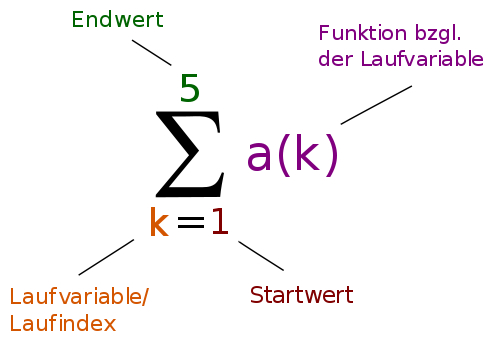
\includegraphics[width = 7 cm]{pictures/summe}
\begin{description}
\item[Endwert] Dieser Wert bestimmt, bis zu welchem Glied die Folge aufsummiert werden soll er kann auch unendlich $\infty$ sein.
\end{description}
\end{minipage}
\begin{minipage}{7 cm}
\begin{description}
\item[Startwert] Dieser Wert ist der erste Wert der Laufvariable und bestimmt somit das erste aufsummierte Folgeglied.
\item[Laufvariable] Diese Variable ist auch Teil des Bildungsgesetzes und wird pro aufsummierten Folgeglieds um 1 erh"oht, bis sie den Endwert erreicht hat.
\item[Funktion bzw. der Laufvariable] Hiermit ist das Bildungsgesetz der urspr"unglichen Folge gemeint.
\end{description}
\end{minipage}

\subsubsection{Endliche Reihen}
Als endliche Reihen werden Reihen bezeichnet, deren Endwert nicht gegen plus Unendlich ($+\infty$) geht. (Ich sage hier mit Absicht "'\textbf{gegen} plus Unendlich geht"', da der Wert Unendlich logischer Weise niemals erreicht werden kann, auch wenn Chuck Norris bis Unendlich z"ahlen kann...)

\subsubsection{Unendliche Reihen}
Was f"ur eine "Uberraschung, dass es bei Unendlichen Reihen nun so ist, dass der Endwert gegen Unendlich geht.
\begin{equation*}
s = \sum\limits_{k=0}^{\infty}g(k)
\end{equation*}

\subsubsection{Monotonie, Beschr"anktheit und Konvergenz}
Genau wie Folgen k"onnen auch Reihen monoton, beschr"ankt und konvergent gegen einen bestimmten Wert sein. Die Definition dieser Begriffe bleibt jedoch genau die selbe, wie auch bei Folgen, weshalb ich sie mir hier spare.

\subsection{Besondere Reihen}
\subsubsection{Konvergierende Reihen und Nullfolgen}
Das Bildungsgesetz jeder konvergierenden Reihe beschreibt eine Nullfolge.
\begin{center}
\textcolor{red}{Anders herum stimmt das allerdings nicht!}
\end{center}
Bekanntestes Gegenbeispiel hierf"ur ist die so genannte \textbf{Harmonische Reihe}:
\begin{equation*}
s_n = \sum\limits_{k=1}^{n}\frac{1}{k}
\end{equation*}
Diese Reihe divergiert gegen Unendlich! Sie wird auch als \textcolor{red}{harmonische Reihe} bezeichnet. Beweis mithilfe einer Absch"atzung:
\begin{align*}
s^{2^{k+}} &= 1 + \frac{1}{2} + \underbrace{\left( \frac{1}{3} + \frac{1}{4} \right)}_{\geq 2 \cdot \frac{1}{4}} + \underbrace{\left( \frac{1}{5} + \ldots + \frac{1}{8} \right)}_{\geq 4 \cdot \frac{1}{8}} + \ldots + \underbrace{\left( \frac{1}{2^k + 1} + \ldots + \frac{1}{2^{k+1}} \right)}_{\geq 2^k \cdot \frac{1}{2^{k + 1}}}\\
&\geq 1 + \frac{1}{2} + 2^{\color{red}1} \cdot \frac{1}{4} + 2^{\color{red}2} \cdot \frac{1}{8} + \ldots + 2^{\color{red}k} \cdot \frac{1}{2^{k+1}} \\
&= 1 + \frac{1}{2} + \underbrace{\frac{1}{2} + \frac{1}{2} + \frac{1}{2} + \ldots + \frac{1}{2}}_{k-\text{mal}}\\
&= 1 + \frac{1}{2} + \frac{1}{2} \cdot k =  1 + \frac{1}{2} + \frac{k}{2} = \frac{3 + k}{2}
\end{align*}

\subsubsection{Geometrische Reihen}
Jede geometrische Reihe kann auch wie folgt dargestellt werden:
\begin{equation*}
\sum\limits_{i=0}^{n} q^i = \begin{cases} \frac{1-q^{n+1}}{1-q} &\mbox{falls } q \neq 1 \\ 
n + 1 & \mbox{sonst.} \end{cases}
\end{equation*}


\subsection{"Ubungen}
\begin{enumerate}
\item Handelt es sich hierbei um eine besondere Art von Reihen?
\begin{itemize}
\item $ s_n = \sum\limits_{i=1}^{\infty} \frac{1}{i} $
\item $ s_n = \sum\limits_{i=1}^{\infty} \frac{1}{i^2} $
\item $ s_n = \sum\limits_{i=1}^{16} 4^i$
\item $ s_n = \sum\limits_{i=2}^{8} i^2 $
\item $ s_n = \sum\limits_{i=0}^{\infty} (-3^i)$
\end{itemize}
\item Sind sie monoton fallend bzw. steigend?
\item Sind die dazugeh"origen Folgen konvergent und/oder beschr"ankt? (Infimum, Supremum und Asymptoten angeben!)
\item Gebe die Ergebnisse der Reihen (au"ser der zweiten) an.
\end{enumerate}

\psection{Beweisverfahren (Bonus)}
\subsection{Direkter Beweis}
Beim direkten Beweis handelt es sich um das \textbf{direkte} Herleiten von Aussagen unter der Annahme von bereits bewiesenen, wahren Aussagen. Wenn wir zeigen können dass 
\begin{equation*}
A_1 \Rightarrow A_2, A_2 \Rightarrow A_3, \ldots A_{n-1} \Rightarrow A_n
\end{equation*}
gilt und $A_1$ eine bereits bewiesene wahre Aussage ist, dann folgt $A_n$. Wir haben also Prämissen, folgern gewisse Schlüsse und gelangen dann zur zu zeigenden Aussage $A_n$.

\subsection{Indirekter Beweis}
Im \textbf{indirekten Beweis} oder auch \textbf{Widerspruchsbeweis} der Aussage $A$ geht man davon aus, dass $A$ nicht zutrifft und zeigt, dass dies aufgrund eines Widerspruchs nicht sein kann. Man geht also zunächst von der Negation aus und versucht auf einen Widerspruch zu stoßen. Angenommen wir wollen $A$ beweisen. Wir wissen
\begin{equation*}
A \lor \neg A
\end{equation*}
ist eine Tautologie. Wir zeigen nun, dass $\neg A \equiv \text{falsch}$, damit muss $A \equiv \text{wahr}$ gelten. Indirekte Beweise sind weniger schön in dem Sinne, dass sie weniger konstruktiv sind. Wir haben einen Widerspruchsannahme, folgern etwas und gelangen zu einem Widerspruch. Dabei kann es sein, dass wir nichts daraus \glqq lernen\grqq \ und wir, bis auf das $A$ gilt, nichts aus dem Beweis \glqq mitnehmen\grqq . Solche Beweise wirken oft \glqq wie vom Himmel gefallen\grqq \ und geben oft kaum Auskunft darüber, welche Idee der Beweisende hatte oder wie und warum er darauf gekommen ist.

\subsubsection{Beispiel}
Das bekannteste Beispiel hierfür ist der Beweis der Aussage:
\begin{equation*}
A:=  \sqrt{2} \text{ ist keine rationale Zahl}
\end{equation*}
Man geht nun davon aus, dass $\sqrt{2}$ eine rationale Zahl ist. Angenommen $\neg A \equiv \text{wahr}$ also angenommen $\sqrt{2}$ ist eine rationale Zahl.
\begin{equation*}
\Rightarrow \exists q, p \in \mathbb{N}:\sqrt{2}=\frac{q}{p},
\end{equation*}
wobei $q$ und $p$ teilerfremd sind (sonst einfach kürzen). Nun quadrieren wir
\begin{equation*}
\Rightarrow 2 = \frac{q^2}{p^2}
\end{equation*}
Nun noch mit $p^2$ multiplizieren
\begin{equation*}
\Rightarrow 2 \cdot p^2 = q^2
\end{equation*}
Da es sich bei $p$ und $q$ um ganze Zahlen handelt, folgt ($\Rightarrow$) dass auch ihre Quadrate ganze Zahlen sind. Eine ganze Zahl mit $2$ multipliziert ist auch wieder eine ganze Zahl. 
\begin{equation*}
\Rightarrow q^2 \in \mathbb{Z}
\end{equation*}
Wenn das Quadrat einer Zahl gerade ist, folgt ($\Rightarrow$) dass auch die Zahl selber gerade ist, deshalb lässt sich $q$ auch folgendermaßen darstellen.
\begin{equation*}
\exists r \in \mathbb{Z} : q = 2 \cdot r
\end{equation*}
Setzt man nun diesen Wert für $q$ oben ein, so erhält man
\begin{equation*}
2 \cdot p^2 = 4 \cdot r^2 \iff p^2 = 2 \cdot r^2
\end{equation*}
Nun sieht man, dass es sich auch bei $p$ um eine ganze, gerade Zahl handelt. Da jede ganze, gerade Zahl den Teiler $2$ hat, besitzen auch $p$ und $q$ den \textbf{gemeinsamen Teiler} 2. Einer unserer Voraussetzungen war allerdings, dass diese beiden Zahlen \textbf{teilerfremd} sind. Wenn wir auf solch einen Widerspruch treffen, so muss zumindest eine unserer Annahmen falsch sein. Die einzige Annahme, welche wir getroffen haben ist jedoch, dass es sich bei Wurzel $2$ um eine rationale Zahl handelt. Diese ist also falsch ($(\neg A) \Rightarrow \text{falsch}$ ist wahr). Damit muss $\neg A \equiv \text{falsch}$ sein und damit $A \equiv \text{wahr}$. Und somit haben wir bewiesen, dass $\sqrt{2}$ keine rationale Zahl ist.

\subsection{Vollständige Induktion}
Das Induktionsprinzip ist sehr natürlich. Es geht im Endeffekt um nichts anderes als ums Zählen. Zählen, so scheint es, liegt in der Natur jedes intelligenten Lebewesens. Stellen Sie sich eine Dominokette vor. Wenn Sie der folgenden Aussage zustimmen können, haben Sie die Induktion im Grunde verstanden:
\begin{center}
Wenn ich den ersten Dominostein umwerfe und zudem gilt, dass wenn ein Dominostein umfällt, folgt, dass sein Nachfolger umfällt, so fallen alle Dominosteine um.
\end{center}
In Form der Prädikatenlogik und unter Annahme, dass wir es mit natürlichen Zahlen zu tun haben, kann man dies wie folgt schreiben
\begin{equation*}
(P(1) \ \land P(x) \Rightarrow P(x+1)) \Rightarrow P(y)
\end{equation*}
Sie müssen nicht zeigen, dass jeder Stein umfällt sondern Sie zeigen dass:
\begin{enumerate}
\item \textbf{Induktionsanfang}: der 1. Stein umfällt und
\item \textbf{Induktionsschluss:} dass wenn Stein $n$ umfällt, fällt Stein $n+1$ um (wenn $n$ nicht der letzte Stein ist)
\end{enumerate}
Allgemeiner nutzen wir dies um Eigenschaften von Objekten zu zeigen, die wir mit einer natürlichen Zahl identifizieren können (Reihen, Folgen, aber auch die $n$-te Ableitung von $f$).

\subsubsection{Beispiel}
Wir wollen nun beweisen:
\begin{equation}
a_{n} = 2 \cdot a_{n-1}; a_1 = 2 \text{ entspricht } b_n = 2^n.
\end{equation}
\begin{enumerate}
\item \textbf{Induktionsanfang:} $n = 1$ (1. Stein): $ a_1 = 2 = 2^1 = b_n$ (passt)
\item \textbf{Induktionsschluss:} $n' = n + 1$ (Achtung nicht $n' = 2$), wir dürfen zudem Annehmen das der $n$-te Stein gefallen ist, dass also $a_n = b_n$ (mehr nicht!).
\begin{align*}
a_{n+1} &\stackrel{\text{nach Def.}}{=} 2 \cdot a_{n+1-1} \\
&=  2 \cdot a_{n} \\
&\stackrel{\text{nach Induktionsanfang}}{=} 2 \cdot b_n \\
&\stackrel{\text{nach Def.}}{=} 2 \cdot 2^n = 2^{n+1} \\
&= b_{n+1}.
\end{align*}
(passt)
\end{enumerate}
Wuhu! Wir haben bewiesen, dass unsere Aussage stimmt.

\subsection{Übungen}
\begin{enumerate}
\item Zeige, dass folgende Aussagen gelten:
\begin{itemize}
\item $\sum\limits_{i=0}^{n} q^i = \frac{1-q^{n+1}}{1-q}$; für $q \neq 1$
\end{itemize}
\end{enumerate}

\end{document}